\documentclass[10pt,a4paper]{article}
\usepackage[utf8]{inputenc}
\usepackage{amsmath}
\usepackage{amsfonts}
\usepackage{amssymb}
\usepackage{graphicx}
\usepackage[table]{xcolor}
\usepackage{float}
\usepackage[table, svgnames, dvipsnames]{xcolor}
\usepackage{makecell, cellspace, caption}
\usepackage{hyperref}
\usepackage[a4paper,
left=20mm,
right=20mm,
top=10mm]{geometry}
\usepackage{titlesec}
\usepackage{enumitem}



\newcommand{\changelocaltocdepth}[1]{%
  \addtocontents{toc}{\protect\setcounter{tocdepth}{#1}}%
  \setcounter{tocdepth}{#1}%
}


\titlespacing*{\subsection}
{0pt}{7ex }{2ex}
\addtolength{\skip\footins}{2pc plus 5pt}

\renewcommand{\baselinestretch}{1.25} 


\author{Nicolò Brandizzi}
\title{Knowledge Representation Summary}
\date{November 2018}

\begin{document}


\begin{titlepage}
    \begin{center}
        \vspace*{1cm}
        
        \Huge
        \textbf{Knowledge Representation Summary}
        
        
        \vspace{1.5cm}
        
        Author:
        \textbf{Nicolò Brandizzi}\\
        \vspace{0.5cm}
        \Large
        Contributors:
        \textbf{}%add contributors here
        
        \vfill
        
        
\includegraphics[width=0.4\textwidth]{images/sapienza_logo.jpg}


        
        \vfill
        
  

        \vspace{0.8cm}
        
        
        \Large
        DIAG\\
        Sapienza\\
        November 2018

    \end{center}
\end{titlepage}


\tableofcontents
\newpage
\begin{abstract}
This is \textbf{free} material! You should not spend money on it.\\
This notes are about the \textit{Knowledge Representation} part taught by professor Daniele Nardi in the Artificial Intelligence class. Everyone is welcome to contribute to this notes in any relevant form, just ask for a pull request and be patient.\\ Remember to add your name under the contributors list in the title page when submitting some changes (if you feel like it).
\end{abstract}

\section{Logic based agents}
A \textbf{knowledge base} [KB] is a set of sentences in a knowledge representation language that express some assertion about the world.\\
We can either:
\begin{itemize}
\item \textit{Tell}: i.e. add new sentences to the KB or
\item \textit{Ask}: i.e. query what is known.
\end{itemize}
We can use both this actions to do \textbf{inference} in which we derive new sentences from old ones.\\

There are two ways of building a KB structure:
\begin{itemize}
\item \textbf{Declarative}: in which the agent is \textit{told} various aspects of the world \footnote{That is the designer add new sentences.} until it is capable of working in the environment.
\item \textbf{Procedural}: which encodes desired behavior directly in the program.
\end{itemize}

Finally an agent can be viewed at:
\begin{itemize}
\item \textit{Knowledge level}, where we specify what the agents knows and what are its goals. Or at
\item \textit{Implementation level}, where we need to specify the data structures used in the KB and the way to manipulate them.
\end{itemize}

\subsection{Logic}
Sentences must follow two principles in order to be considered \textit{correct}:
\begin{itemize}
\item \textbf{Syntax} holds when a sentence is \textit{well formed}, e.g. in mathematics "$x+y=4$" is correct while "$x3y +=$" is not.
\item \textbf{Semantic}  that defines the \textit{truth} of a sentence in respect to each possible world. For example the sentence $x+y=4$ is true in a world where $x=2,y=2$ but false when $x=1,y=4$.
\end{itemize}

Other than saying \textit{each possible world} when referring to the KB, we can use the word \textbf{interpretation}. Whereas possible worlds might be thought of as (potentially) real environments that the agent might or might not be in, interpretations are mathematical abstractions, each of which simply fixes the truth or falsehood of every relevant sentence.\\

Moreover a \textbf{model} $m$ is an interpretation of a sentence $\alpha$ if $\alpha$ is true in $m$ \footnote{Here the Russell-Norvig has a different concept of \textit{model} which is equal to the above \textit{interpretation (= each possible world = model)} . But Nardi prefer to make the distinction between the two, so we will go with the Nardi flow (\textit{each possible world=interpretation $\neq$ model=true interpretation}).}. Given a set of the models of $\alpha$, $M(\alpha)$, we can derive the concept of \textit{entailment}:\\
A KB \textit{entails} a sentence $\alpha$ \footnote{That is the sentence $\alpha$ follows logically/is derived from KB.} if and only if, in every interpretation in which the KB is true \footnote{That is in every \textit{model} of the KB.}, $\alpha$ is also true:
\[KB \models \alpha \Leftrightarrow M(KB) \subseteq M(\alpha)\]
Note that $ M(KB) \subseteq M(\alpha)$ means that KB is a \textit{stronger assertion} than $\alpha$ since it \textit{rules out} more interpretation or possible worlds \footnote{There are less models in KB than in $\alpha$.}.

\paragraph{Example} Lets make an example to better understand this concepts.\\
We have the following sentences: 
\begin{itemize}
\item $\alpha=$ Overwatch is better than Fortnite.
\item $\beta=$ Everything is better than Diablo immortal \footnote{Don't you have phones?}.
\end{itemize}
Our KB is equal to $KB=\alpha \wedge \beta$, that is the KB knows that \textit{Overwatch is better than Fortnite \textbf{and} that Diablo immortal sucks}. We want to know:
\[KB \models \beta\]
i.e. we can derive from KB that Diablo immortal sucks.\\
We first need to check if $M(KB) \subseteq M(\beta)$, in other words if the KB has fewer true interpretation \footnote{Models.} than $\beta$. We know that the entailment holds since:
\begin{itemize}
\item The KB has two independent sentences, $\alpha,\beta$, correlated by an \textit{and} logic relationship, which result in fewer models.
\item  We are asking the KB for the truth of a sentence which is directly part of the KB itself; so that the set of models $M(KB)$ is a \textit{subset} of $M(\beta)$.
\end{itemize}

\paragraph{Model checking}
\label{sec:model_checking}
To know if $KB \models \beta$ we need to prove that $M(KB) \subseteq M(\beta)$. This can be done by \textbf{model checking}, that is enumerating all the possible interpretation where $KB$ is true and check if those are also models of $\beta$ \footnote{This is a direct implementation of the definition of entailment.}. For the above example we have:

\begin{table}[H]
\centering
    \begin{tabular}{|l|l|l|}
        \hline
        ~                              & KB    & \beta \\ \hline
        \alpha \wedge \beta            & \cellcolor{blue!25} True  & \cellcolor{blue!25} True  \\ 
        \neg \alpha \wedge \beta     & False & \cellcolor{blue!25} True  \\ 
        \alpha \wedge \neg \beta       & False & False \\ 
        \neg \alpha \wedge \neg \beta  & False & False \\
        \hline
    \end{tabular}
    \caption{Model checking for $KB\models\beta$}
\end{table}

\paragraph{Deduction} 
To better understand the difference between entailment and inference we should think of the \textit{set of all consequences} of KB as a haystack and $\beta$ as a needle. Entailment is like the needle being in the haystack; inference is like finding it.

Another way of computing the knowledge entailed by a KB is by a \textbf{deduction procedure}:
\[KB \vdash_i \beta\]
Which denotes that $\beta$ can be driven from KB by an \textbf{inference algorithm} $i$. 

\paragraph{Sound and Completeness} Given an inference algorithm $i$, if $i$ derives \textbf{only entailed} sentences from KB then it is considered \textbf{sound} \footnote{Or truth preserving.}, otherwise $i$ would make things up as it goes along (discovering of non-existing needles).\\
On the other hand \textbf{completeness} is also desirable: an inference algorithm is complete if it can derive any sentence that is entailed. For real haystacks, which are finite in extent, it seems obvious that a systematic examination can always decide whether the needle is in the haystack. For many knowledge bases, however, the haystack of consequences is infinite, and completeness becomes an important issue.

\paragraph{Difference between $\models$ and $\vdash$}
Having 
\begin{itemize}
\item $KB\models \alpha$
\item $KB \vdash \alpha$
\end{itemize}
The first symbol $\models$  is called \textbf{entailment} and means that $\alpha$ must be true in all of KB's models, that is KB  are true when $\alpha$'s interpretations are true \footnote{We can have some models of $\alpha$ which are not model in KB.}.\\
The other symbol $\vdash$ is read \textbf{derives} (KB derives $\alpha$) it can be joint with a sign denoting an inference rule, such as $KB \vdash_{MP}\alpha$ \footnote{Modus Ponens Section \ref{subsec:modusPonens}.} or $KB \vdash_{R}\alpha$ \footnote{Resolution Section \ref{sec:resolution}.} or both $KB \vdash_{R,MP}\alpha$. You can even ignore the set of inference rules and just write $KB \vdash\alpha$, in this case you are saying that \textit{it must exist a derivation \footnote{Obtained with some inference rule.} so that $\alpha$ is the last element of the chain}. You can verify the entailment with the derivation if and only if the inference rules you are applying are sound and complete.


\paragraph{Difference between \textit{deduction} and \textit{inference}}
Broadly speaking they are the same thing.\\
More specifically, the \textit{deduction} is always referred to as a syntactic derivation, while \textit{inference} is a more generic  term which means that starting from KB we can conclude $\alpha$. So \textit{deduction} is tied to the $\vdash$ symbol, while \textit{infer} is more generic and can be used in both $\vdash, \models$

\newpage
\section{Propositional Logic}
Propositional logic is the simplest logic! \footnote{Not to understand...}

\paragraph{Syntax}
\label{par:syntax}
An \textbf{atomic sentence} is made of \textit{one} \textbf{propositional symbol} (for example $S$), which can be either \textit{True or False}.\\
\textit{True and False} are propositional symbols that are always True/False.\\
\textbf{Complex sentences} are propositional symbols joint together by the following \textbf{logical connective} (Figure \ref{fig:prop_synt}) :
\begin{itemize}
\item $\neg$ (not): $\neg S$ is the \textbf{negation} of $S$.
\item $\wedge$ (and): $S_1\wedge S_2$ is a \textbf{conjunction}.
\item $\vee$ (and): $S_1\vee S_2$ is a \textbf{disjunction}.
\item $\Rightarrow$ (implies): $S_1\Rightarrow S_2$ is an \textbf{implication}, where $S_1$ is the \textit{antecedent/premise} and $S_2$ is the \textit{consequent/conclusion}. Implication are known as \textbf{if-then} statement \footnote{If premise then conclusion.}.
\item $\Leftrightarrow$ (if and only if): $S_1\Leftrightarrow S_2$ is a \textbf{biconditional}.
\end{itemize}

\begin{figure}[H]
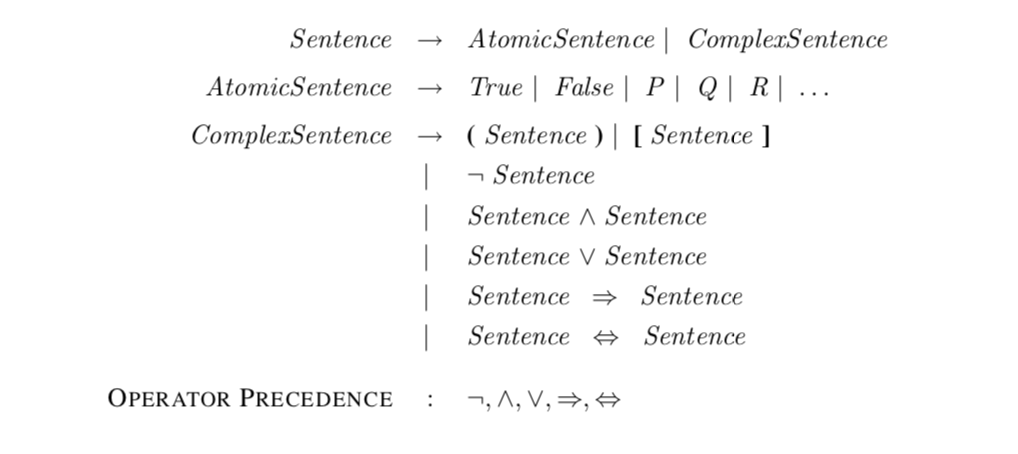
\includegraphics[scale=0.7]{images/prop_syntax.png}
\caption{Syntax summary for propositional logic}
\label{fig:prop_synt}
\end{figure}

\paragraph{Semantic}
The semantic defines the truth of a sentence in respect to a particular interpretation, that assign a truth value to every propositional symbol (Figure \ref{fig:truth_table}).

\begin{figure}[H]
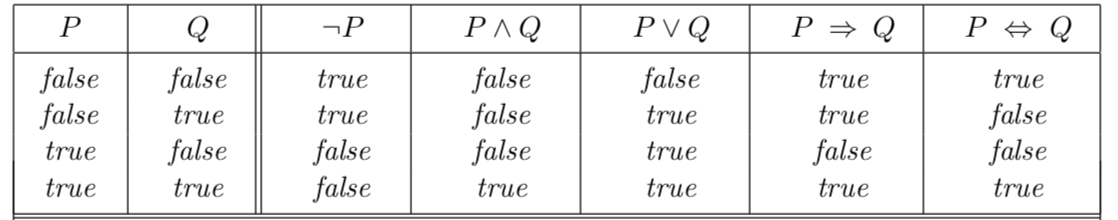
\includegraphics[scale=0.7]{images/truth_table.png}
\caption{Truth Table for propositional logic.}
\label{fig:truth_table}
\end{figure}

For  what regard the \textit{implies} symbol ($P \Rightarrow Q$) we need to specify that:
\begin{itemize}
\item It \textit{does not} need to have any causal/relevance link between the antecedent and the consequent. For example \textit{'5 id odd implies Tokyo is the capital of Japan'} is syntactically correct.
\item Any implication is true whenever the antecedent is false. This because we are saying \textit{'If P is true, then I am claiming that Q is true. Otherwise I am making no claim'}.
\item The only way for $P \Rightarrow Q$ to be false is if $P$ is true and $Q$ is false.
\end{itemize}


\paragraph{Inference}
Our goal is to prove that
\[KB \models \alpha\]
With the model checking approach we just need to enumerate all the possible interpretation and check that, when there is a model of KB then there is also a model of $\alpha$. This is done by assigning either \textit{true} or \textit{false} to every propositional symbol in any interpretation. But given $n$ symbols there are $2^n$ interpretations, thus the time complexity is $O(2^n)$, while the space complexity is $O(n)$ since we're using a depth-first approach. 

\subsection{Theorem Proving}
We can use a technique known as \textit{theorem proving} that consist in applying rules of inference directly to the sentences in our KB to construct a proof of the desired sentence without consulting models. If the number of models is large but the length of the proof is short, then theorem proving can be more efficient than model checking. We first need to introduce some concepts.

\paragraph{Logical equivalence} Two sentences $\alpha$ and $\beta$ are logically equivalent if they are true in the same set of interpretations, i.e. they have the \textbf{same set of models}. We write this as $\alpha \equiv \beta$. We can formalize this propriety by writing:
\[\alpha \equiv \beta \Longleftrightarrow \alpha \models \beta \wedge \beta \models \alpha\]
Following there are some standard logic equivalences (Figure \ref{fig:logic_equivalences}):


\begin{figure}[H]
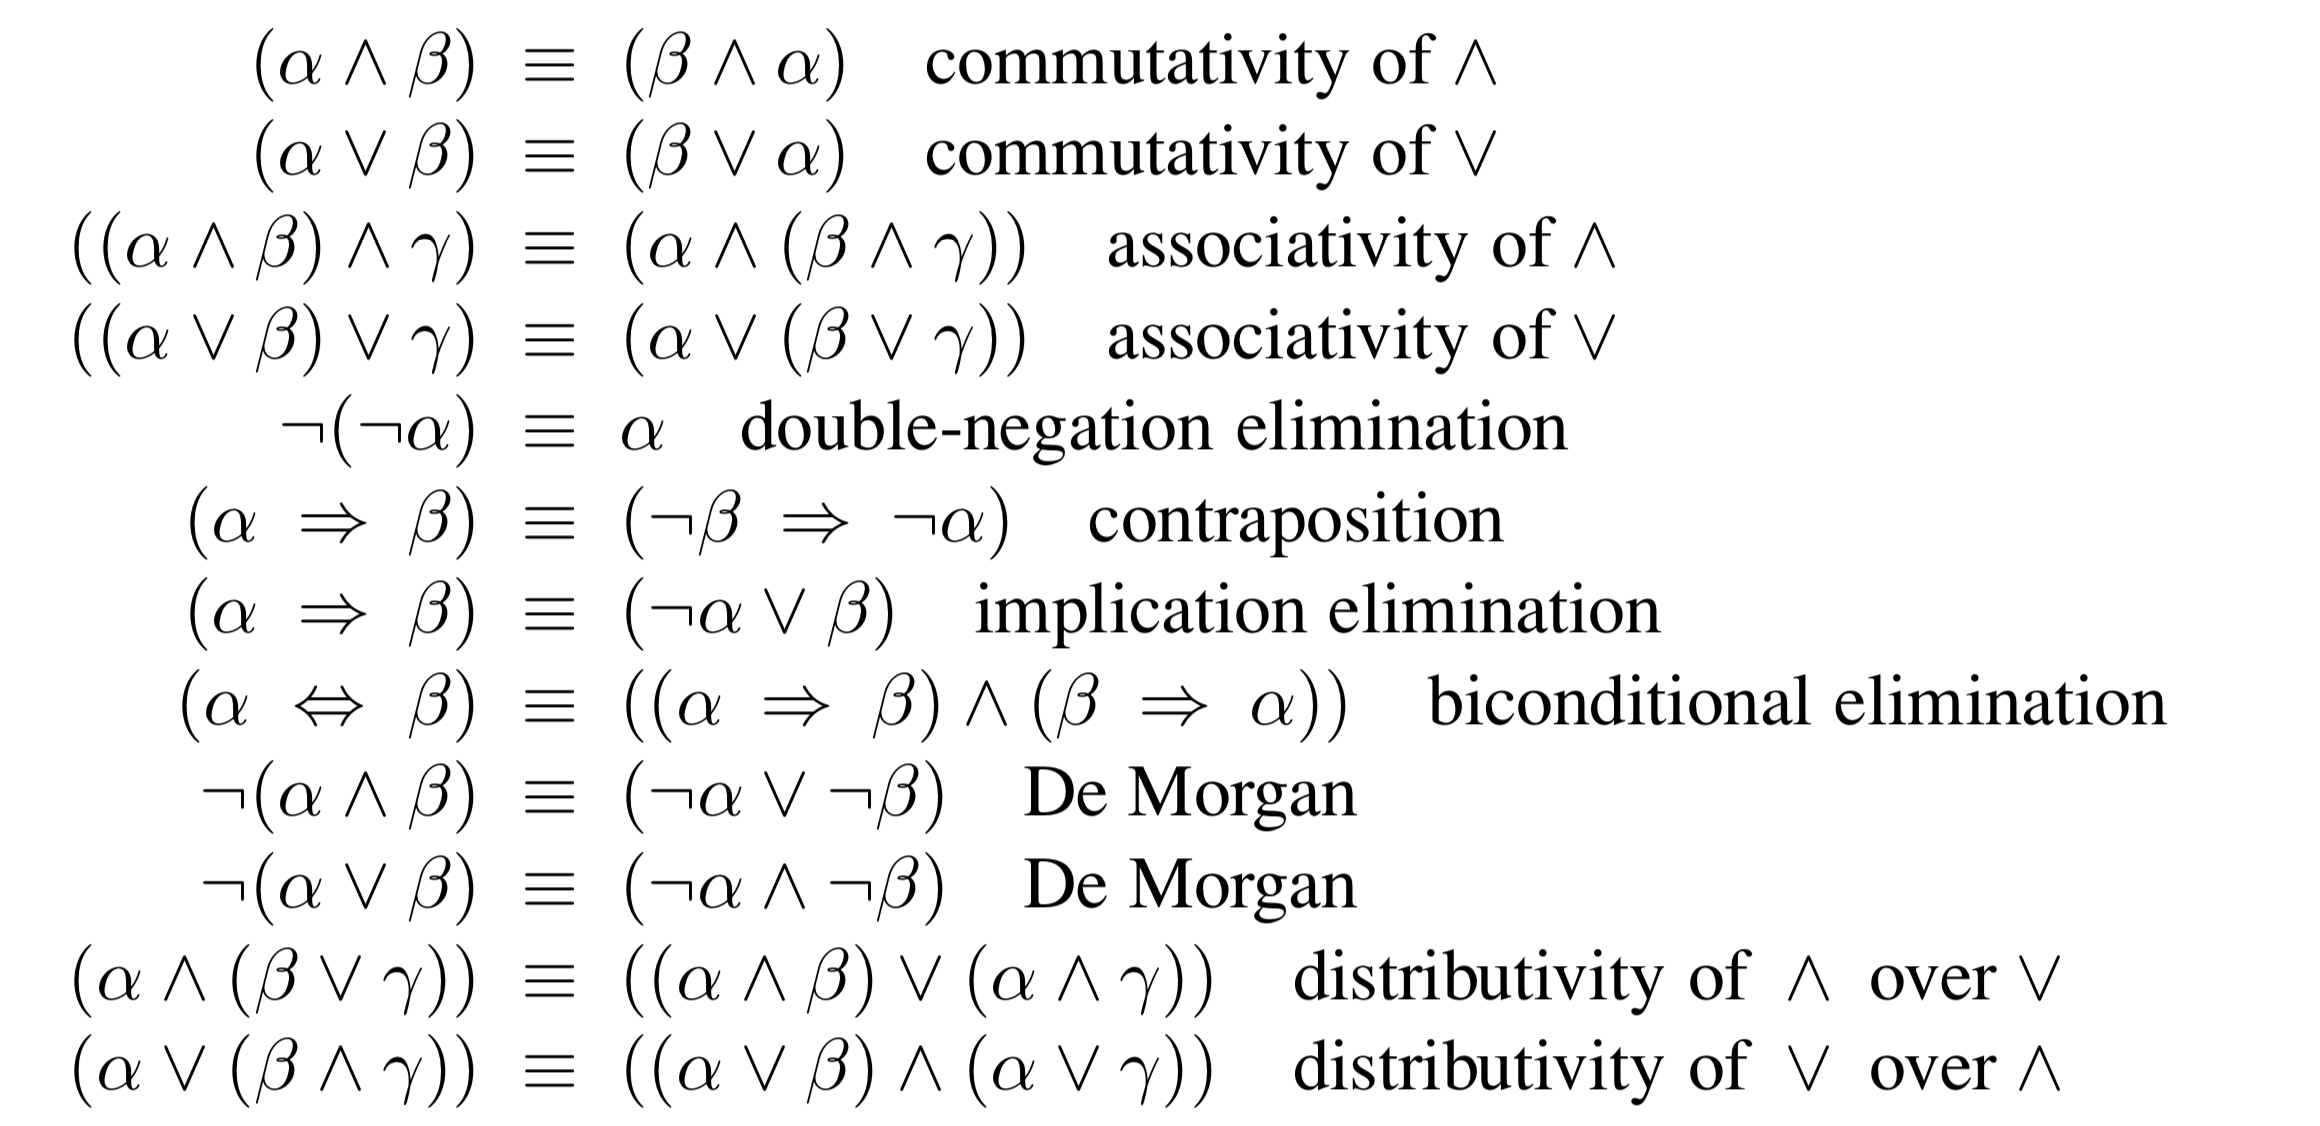
\includegraphics[scale=0.3]{images/equivalences.png}
\caption{Standard logic equivalences.}
\label{fig:logic_equivalences}
\end{figure}


\paragraph{Validity}
\label{sec:validity}
A sentence is \textit{valid} if it is true in all interpretations \footnote{Also known as tautologies.}. For example: $A \vee \neg A$, $True$, $A \Rightarrow A$...\\
Validity can be tied to the deduction problem in the following way:\\
\textit{For every sentences $\alpha$ and $\beta$, $\alpha \models \beta$ if and only if the sentence $\alpha \Rightarrow \beta$ is valid}.

\paragraph{Satisfiability}
\label{sec:satisfiability}
A sentence is \textbf{satisfiable} \footnote{This problem is called SAT and it has been shown to be NP-complete.} if it is true in \textit{some} interpretation, i.e. it has some models. A sentence can be proved to be satisfiable by enumerating the possible implementations until a model is found \footnote{Model checking technique.}.\\
We can say that:
\begin{itemize}
\item \textit{$\alpha$ is valid iff $\neg \alpha$ is unsatisfiable}, or
\item \textit{$\alpha$ is satisfiable iff $\neg \alpha$ is not valid}.
\end{itemize}
Hence we can give another interpretation for entailment:
\[\alpha \models \beta \Longleftrightarrow (\alpha \wedge \neg \beta)\quad is \quad unsatisfiable\]
Which is also known as the \textbf{reductio ad absurdum} (proof by contradiction).


\paragraph{Consistency}
\label{sec:consistency}
A knowledge base KB is consistent iff its negation is not a tautology \footnote{A tautology  is a formula or assertion that is true in every possible interpretation}.
That is, KB is inconsistent (not consistent) iff there is no interpretation which entails KB.\\
Example of an inconsistent knowledge base:
\[KB=\lbrace a, \neg a \rbrace\]


\subsubsection{Deduction in Propositional Logic}
\label{subsubsec:deduction}
We can use \textit{inference rules} to derive a proof \footnote{A proof is a chain of conclusion which leads to a desired goal.} of the interpretation truthfulness.
The idea behind finding a proof rather than using model checking is that the proof can ignore irrelevant proposition, no matter how many of them there are.\\
Usually this kind of rules are written in the form:
\[\frac{premisies}{conclusions}=\frac{A_1,A_2,...,A_n}{A}\]

Suppose we want to derive some formula \footnote{Or sentence.} $\alpha$ from the KB\footnote{Which is a set of formulas.} ($KB \vdash \alpha$), there must be a sequence of formulas $\alpha_1,...,\alpha_n$ such that:
\begin{itemize}
\item For every $i$ between $1...n$ either:
	\begin{itemize}
	\item $\alpha_i\in KB$, that is the formula $\alpha_i$ is in the KB. Or
	\item  $\alpha_i$ is a \textit{direct derivation} of $\alpha_{i-k},\ k\in [1,i-1]$ \footnote{$\alpha_i$  is a direct derivation of the previous formulas. In general $\alpha_i$ can depend on any subset of previous $\alpha$, it depends on the resolution rule used. }
	\end{itemize}
\item $\alpha=\alpha_n$, the chain of direct derivations brings to the formula we want to infer.
\end{itemize} 
Hence we can say that $\alpha_1,...,\alpha_n$ is a proof of $\alpha$ from the KB.
Finding a proof for a formula can implemented as a search where:
\begin{itemize}
\item \textit{Initial State}: is the KB  .
\item \textit{Operators}: are \textit{inference rules} (mentioned earlier).
\item \textit{Final state}: is the formula to be proven.

\end{itemize}



\paragraph{Basic proprieties}
We need to describe the proprieties of a inferring method $\mathcal{R}$ given a set of formulas $KB$ and a formula $A$. It is important to understand that by writing $\models A$ we are referring to the truthfulness of $A$ in all its interpretation, thus referring to the \textit{validity} of $A$.
\begin{itemize}
\item First we need to prove that an infer rule $\mathcal{R}$ is \textbf{sound}, to do so we need to prove that $A$ is \textbf{valid} given the fact that it can be derived with $\vdash_{\mathcal{R}}$.\\ 
First thing is to notice that there is no KB before the symbol since we want to prove $A$ being valid  regardless of the existence of any KB \footnote{That is a formula which is true in all models, for example $A \vee \neg A$.}.\\
But if we can derive $A$ with a deduction $\vdash$ then $A$ must be valid, so $\mathcal{R}$ is \textbf{sound} and we have: $KB \vdash_{\mathcal{R}} A$ implies $KB \models A$.
\item On the other hand, if $A$ is valid then it exist a derivation $\vdash_{\mathcal{R}} $ than let me derive it, so that $KB \models A$ implies $KB \vdash_{\mathcal{R}} A$, thus  $\mathcal{R}$ is \textbf{complete}.
\end{itemize}

\subsubsection{Inference and proof}
\label{subsec:modusPonens}

First thing first the truth tables we cited before are not associated with the inference rules. They are associated with the formulas! So you cannot apply any truth table to Modus Ponens, And Elimination and Resolution since it does not make sense.\\

Moreover atom and literal are the two basic elements for the construction of the formulae, in propositional logic $A$ is a propositional variable. But since we can have bot $A$ and $\neg A$ we say that $A$ is a literal which can be positive or negative.\\

The syntax (Section \ref{par:syntax}) allows you to build a formula regardless of the amount of free variable \footnote{This is use in general cases.}, when you have a formula with no free variables then its called a \textbf{sentence}. For example if we say:
\[A\wedge B \Rightarrow C\]
then its a formula, but if we associate a meaning to each literals:
\[Student \wedge SteamSales \Rightarrow Happy\]
Then it becomes a sentence.\\

On the other hand we used atom to indicate a formula for the estimations of predicates that has a predicates and some arguments. While in the propositional logic we have the propositional variable as a base element and an atom is a literal, in First Order Logic we have atoms.


\paragraph{Modus Ponens} We can ether use Modus Ponens:
\[\frac{\alpha \Rightarrow \beta,\quad \alpha}{\beta}\]
Which given $\alpha \Rightarrow \beta$ and $\alpha$ it can infer $\beta$. For example
\[\frac{man \Rightarrow mortal,\quad man}{mortal}\]
or
\[\Gamma =\lbrace feline \Rightarrow animal, cat \Rightarrow feline, cat \rbrace\]
Result in 
\[\Gamma \vdash_{MP} animal\]
Which mean that \textit{animal} can be derived from $\Gamma$ using the inference algorithm MP (Modus Ponens).\\

\paragraph{And Elimination}On the other hand we can use and elimination:
\[\frac{\alpha\wedge\beta}{\alpha}\]
more in general:
\[\frac{\alpha_1\wedge\alpha_2\wedge...\wedge \alpha_n}{\alpha_i}\]
Which works for any chain of conjunction and means that \textit{"if the rule $A=\lbrace\alpha_1\wedge\alpha_2\wedge...\wedge \alpha_n\rbrace$ is true, then for any $\alpha_i \in A$, $\alpha_i$ must be true as well"}, since we have an \textit{and} logical chain.\\

\paragraph{Monotonicity}
Finally \textbf{monotonicity} is the propriety of logical system  which says that the set of entailed sentences can only increase as information is added to the knowledge base:
\[if\ KB\models \alpha\ then \ KB\wedge\beta\models\alpha\]
Which means that inference rules can be applied whenever suitable premises are found in the KB; conclusion of the rule must follow regardless of what else is in the knowledge base \footnote{Nonmonotonic logics, which violate the monotonicity property, capture a common property of human reasoning: changing one's mind.}.

\paragraph{Inference rules}
We can use any of the equivalences from Figure \ref{fig:logic_equivalences} as inference rules, for example:
\[\frac{\alpha \Leftrightarrow \beta }{(\alpha \Rightarrow \beta)\wedge(\beta\Rightarrow\alpha)}\quad and\quad \frac{(\alpha \Rightarrow \beta)\wedge(\beta\Rightarrow\alpha)}{\alpha \Leftrightarrow \beta }\]

\subsection{Resolution}
\label{sec:resolution}
So far we did not provide any algorithm which can be considered \textbf{complete}, since the lack of some \textit{inference rules} may prevent the algorithm from reaching the goal. So we introduce the inference rule called \textbf{resolution} that yields a complete inference algorithm when coupled with any complete search algorithm (Section \ref{subsec:search_alg}).

\paragraph{Definitions}
Following there are some definitions:
\begin{itemize}
\item \textit{Formula}: is a set of literals joint by some logic connectives (e.g. a complex sentence).
\item \textit{Literals}: can be either one propositional symbol (or atom) or a negated atom. They are the same as an atomic formulae that is a formula that contains no logical connectives.
\item \textit{Clause}, is a \textit{disjunction} of literals, for example $L_1\vee L_2\vee...\vee L_n$
\item Moreover we introduce the constants $\bot$ and $\top$, that are \textit{False} and \textit{True} respectively.

\end{itemize}





\subsubsection{Conjunctive Normal Form [CNF]}
\label{subsec:cnf}

First thing first note that if we have a KB on which we \textit{can} use Modus Ponens \textit{then} we can use Resolution too. On the other hand if we can use Resolution then we may be not able to use Modus Ponent, since generalize Modus Ponens can be only used for definite horn clauses.



\paragraph{Definition}
The key idea is that: \textit{every sentence of propositional logic is logically equivalent to a conjunction of clauses} ($Formula\equiv CNF(Formula)$) ; hence sentences expressed as a conjunction of clauses are said to be in CNF. You can either preserve equivalence when converting to CNF, but the number of clauses will be $2^n$, where $n$ is the number of literals; or you can preserve \textit{satisfiability} introducing new literals and linearly increase the size of the formula.\\



\paragraph{Example}
Let's make an example using:
\[A \Leftrightarrow (B \vee C)\]
In the following steps we make use of the formulae in Figure \ref{fig:logic_equivalences}

\begin{enumerate}
\item Use biconditional elimination and get: \\$(A \Rightarrow (B \vee C))\wedge((B \vee C)\Rightarrow A)$
\item Use implication elimination end get :\\$(\neg A \vee B \vee C)\wedge(\neg(B\vee C)\vee A)$
\item CFN requires the negation to be applied only to literals \footnote{When a sentence has negation symbols applied directly to literal then it is in \textbf{Negation normal form} [NNF]. For example $\neg(A\vee B)$ is not in NNF while $\neg A \wedge \neg B$ is.}, hence we need to use the De Morgan formula to move $\neg$ inwards: \\$(\neg A \vee B \vee C)\wedge((\neg B\wedge \neg C)\vee A)$
\item Finally we use the distributive law of $\vee$ over $\wedge$ and get:\\
$(\neg A \vee B \vee C)\wedge(\neg B \vee A)\wedge(\neg C \vee A)$
\end{enumerate}


\paragraph{Alpha-Beta Formulas}
There are some cases in which we need to separate dis/conjunction depending on the following formulas:
\begin{table}[H]
    \begin{tabular}{|l|l|l|l|}
        \hline
        C=\lbrace \alpha \rbrace     & C_1=\lbrace \alpha_1 \rbrace,C_2=\lbrace \alpha_2 \rbrace & C=\lbrace \beta \rbrace & C=\lbrace \beta_1, \beta_2\rbrace \\ \hline\hline
        \alpha =A \wedge B           & \alpha_1 = A,\ \alpha_2= B                                & \beta=A\vee B           & \beta_1= A ,\ \beta_2=B           \\ \hline
        \alpha =\neg(A\vee B)        & \alpha_1 =\neg A,\ \alpha_2= \neg B                       & \beta=A \Rightarrow B   & \beta_1=\neg A,\ \beta_2= B       \\ \hline
        \alpha =\neg(A\Rightarrow B) & \alpha_1=A,\ \alpha_2= \neg B                             & \beta=\neg(A\wedge B)   & \beta_1=\neg A,\ \beta_2= \neg B  \\
        \hline
    \end{tabular}
\caption{Alpha-Beta formulas for CNF}
\label{tab:alpha-beta}
\end{table}
As you can see from Table \ref{tab:alpha-beta} the alpha formulas result into two clauses \footnote{That is because there is a conjunction symbol. } $C_1,C_2$, while the beta formulas terminate in a single clause $C$ with two formulas \footnote{Note that I said formulas and not literals since both $\alpha_1,\alpha_2,\beta_1,\beta_2$ can be further simplified if they are not literals.}.

\paragraph{Algorithm}
Given a formula $F$ the algorithm for having the latter in CNF is the following:

\begin{enumerate}
\item Let $I=\lbrace F \rbrace$\footnote{The braces indicates that the $I$ is a set of clauses which will be joint by conjunctions.} be the initial state.
\item At the step $n+1$ we have that $I=\lbrace D_1,...,D_n \rbrace$ where $D_i$ is a disjunction containing some formulas $\lbrace A_1^i,...,A_k^i\rbrace$. 
\item If $A^i_j$ is not a literal then choose $D_i$ and do the following $\forall X_j \in D_i$:

	\begin{itemize}
	
	\item if $X_j$ is $\neg \top$ then replace it with $\bot$.
	\item if $X_j$ is $\neg \bot$ then replace it with $\top$.
	\item if $X_j$ is $\neg \neg X_j$ then replace it with $X_j$.
	\item if $X_j$ is $\beta$ formula then replace it with $\beta_1,\beta_2$.
	\item if $X_j$ is $alpha$ formula then replace $D_i$ with two clauses $D_i^1,D_i^2$ and add them to $I$. 

	\end{itemize}
	
\item Continue until every $D_i$ is made of literals.

\end{enumerate}


\paragraph{Expansion rules}
Finally note that the above rules can be written in the form of \textit{expansion rules} \footnote{Using the form introduced in Section \ref{subsubsec:deduction}.}:
\[\frac{\neg\neg A}{A}\quad \frac{\neg \top}{\bot}\quad \frac{\neg \bot}{\top}\quad \frac{\beta}{\beta_1,\beta_2}\quad \frac{\alpha}{\alpha_1 |\alpha_2}\]

\paragraph{Another Example}
Given the formula:
\[(P\Rightarrow (Q \Rightarrow(S\vee T)))\Rightarrow(T\Rightarrow Q)\]
We have that:
\begin{enumerate}
\item Use implication elimination (from now on it will be taken for granted) and get:
\[\neg(P\Rightarrow (Q \Rightarrow(S\vee T)))\vee(T\Rightarrow Q)\]
\item Use $\beta$ rule on disjunction:
\[C=\lbrace \beta_1= \neg(P\Rightarrow (Q \Rightarrow(S\vee T))),\beta_2=(T\Rightarrow Q)\rbrace\]
\item Use $\alpha$ rule on $\beta_1$ (negation of implication) and get:
\[C_1=\lbrace P,(T\Rightarrow Q)\rbrace,\quad C_2=\lbrace \neg  (Q \Rightarrow(S\vee T)),(T\Rightarrow Q)\rbrace \]
\item Use $\beta$ rule on $C_1$:
\[C_1=\lbrace P,\neg T, Q\rbrace,\quad C_2=\lbrace \neg  (Q \Rightarrow(S\vee T)),(T\Rightarrow Q)\rbrace \]
\item Use $\beta$ rule on $C_2$:
\[C_1=\lbrace P,\neg T, Q\rbrace,\quad C_2=\lbrace \neg  (Q \Rightarrow(S\vee T)),\neg T, Q\rbrace \]
\item Use $\alpha$ rule on $C_2$:
\[C_1=\lbrace P,\neg T, Q\rbrace,\quad C_2=\lbrace \neg  Q ,\neg T, Q\rbrace\quad C_3=\lbrace \neg(S \vee T),\neg T, Q\rbrace \]
\item Use $\alpha$ rule on $C_3$:
\[C_1=\lbrace P,\neg T, Q\rbrace,\quad C_2=\lbrace \neg  Q ,\neg T, Q\rbrace\quad C_3=\lbrace \neg S,\neg T, Q\rbrace\quad C_4=\lbrace \neg T,\neg T, Q\rbrace
\]
\end{enumerate}

\subsubsection{Horn clause}
\label{subsubsec:horn}

\paragraph{Definitions}
The definition for understanding Horn clauses are both reported in Figure \ref{fig:clauses} as well as in the following list:
\begin{itemize}
\item \textit{Definite clause}: is a disjunction of literals of which \textit{exactly one is positive}. For example:\[(\neg L_1 \vee \neg L_2 \vee L_3)\]
\item \textit{Goal clause}: is a disjunction of literals of which \textit{none is positive}. For example:\[(\neg L_4 \vee \neg L_5 \vee \neg L_6)\]
\item \textit{Horn clause}: is a disjunction of literals of which \textit{at most one is positive}. So you can either have \textit{definite clauses} or \textit{goal clauses}. For example:\[(\neg L_1 \vee \neg L_2 \vee L_3)\quad or\quad (\neg L_4 \vee \neg L_5 \vee \neg L_6)\]
\item \textit{Horn Form}: a KB is in Horn form if it is a conjunction of Horn clauses. For example:

	\begin{enumerate}
	\item $C \wedge (B\Rightarrow A)\wedge(C\wedge D\Rightarrow B)$
	\item $C \wedge (\neg B \vee A)\wedge(\neg(C\wedge D)\vee B)$
	\item $C \wedge (\neg B \vee A)\wedge(\neg C\vee \neg D \vee B)$
	\end{enumerate}
	
\end{itemize}

\paragraph{Motivation}
So why are we interested in definite/goal/Horne clauses?\\
\begin{itemize}
\item When we have a definite clause we can write it as an implication of conjunctions. For example:
\[(\neg L_1 \vee \neg L_2 \vee L_3)\quad becomes\quad (L_1 \wedge L_2)\Rightarrow L_3\]
In this case the premise is called the \textit{body} and the conclusion is called \textit{head}. Moreover a single positive literal is a \textit{fact} \footnote{Since a single literal can be viewed as a disjunction of one literal.}.
\item what is the advantage of having a goal clause??????????
\item Moreover inference in horn clauses can be done with the forward/backward chaining algorithm (Section \ref{subsec:chaining}).
\item Finally deciding entailment with Horn clauses can be done in time that is linear in the size of the knowledge base.




\end{itemize}

\begin{figure}[H]
\centering
\fbox{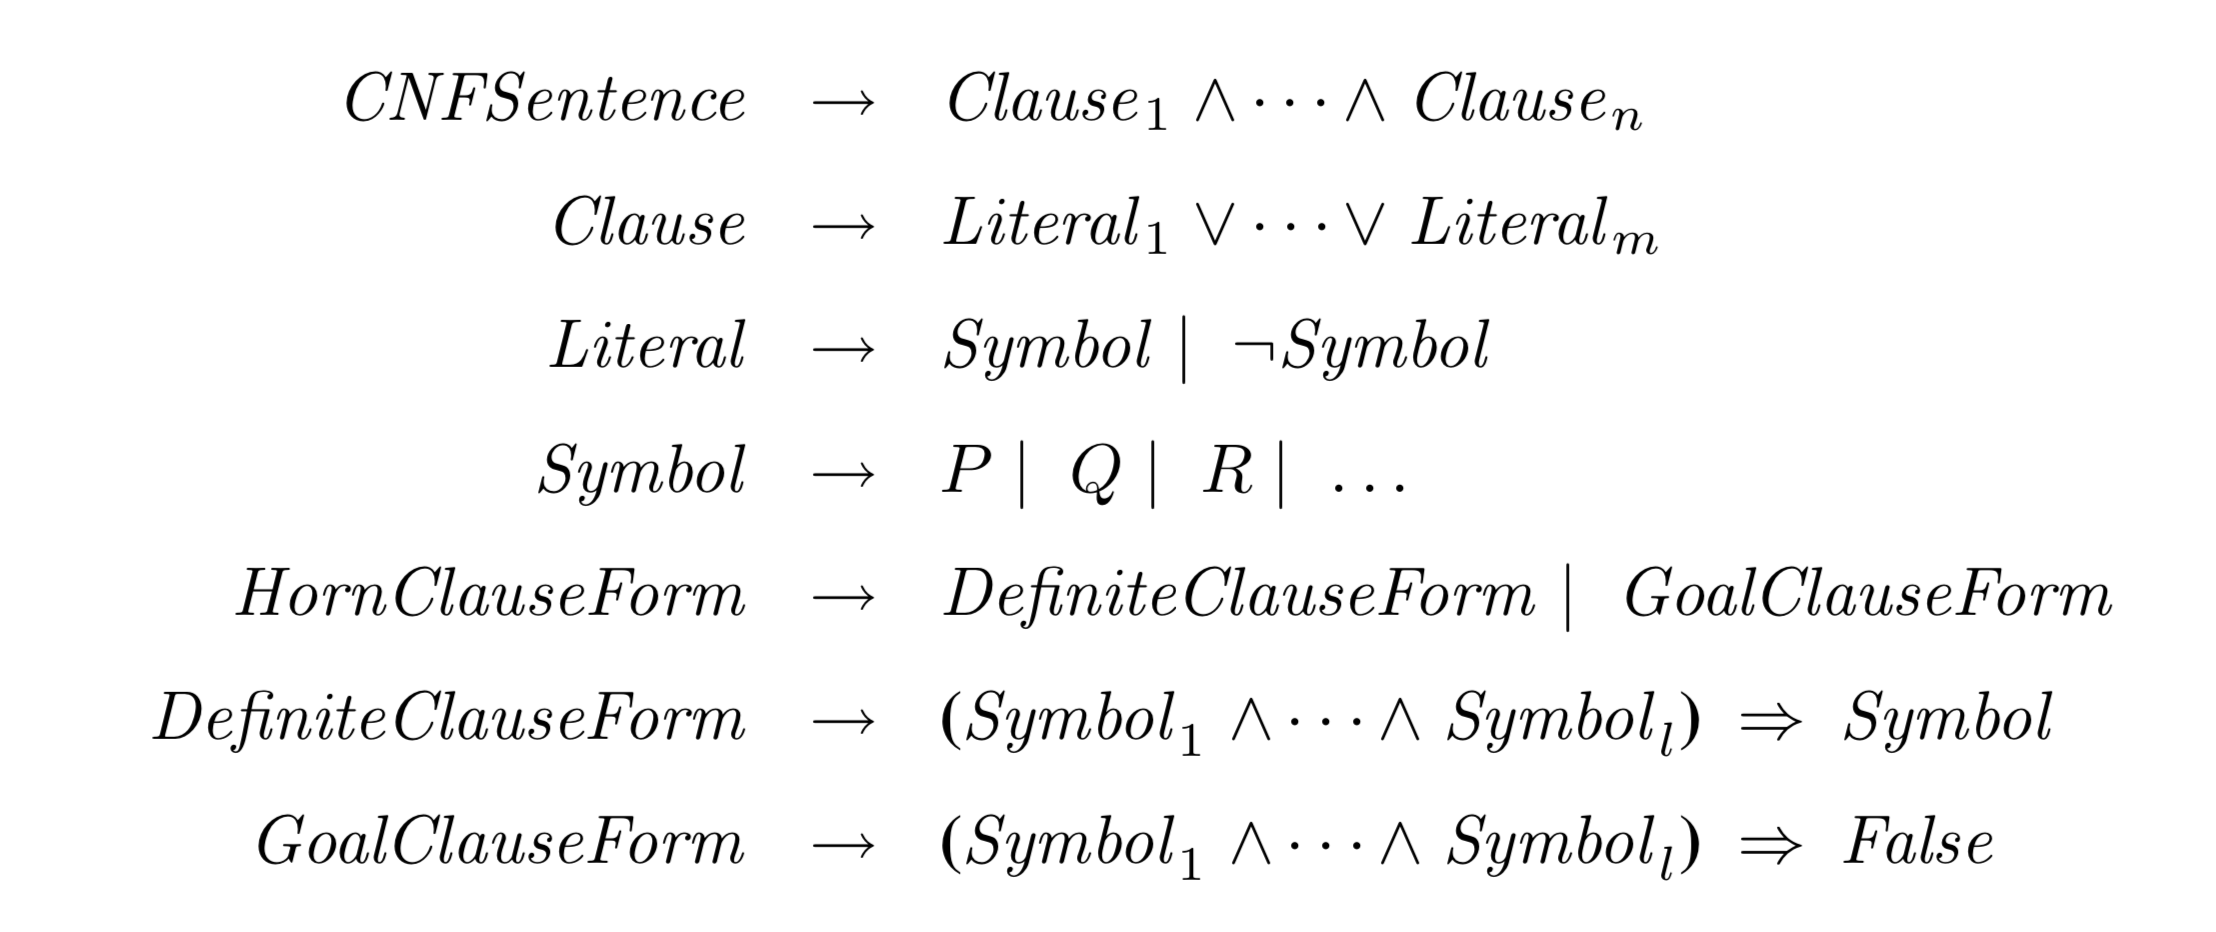
\includegraphics[scale=0.3]{images/horn_clause.png}}
\caption{Different types of clauses}
\label{fig:clauses}
\end{figure}

\subsubsection{Propositional Resolution }
\label{subsubsec:prop_resolution}
The key idea of the propositional resolution is that if I have two clauses $C_1,C_2$ \footnote{You should know by now that a clause is a disjunction of literals.} and one literal $L$ that appears with different sign in both $L \in C_1\ ,\neg L \in C_2$, then I can generate a new clause by joining $C_1 \vee C_2$ and removing $L,\neg L$ from them. That is because if I have a clause where a symbol appears with both sign, e.g. $C_3=L_1 \vee L_2 \vee \neg L_1$, then every interpretation I can give to $L_1$ will be indifferent since it will result in a model. 

\paragraph{English Example} Consider the following KB, with two clauses, trying to understand why can't I play Overwatch on Monday:
\begin{itemize}
\item $C_1$=\textit{"There is an exam the next day"} or \textit{"My pc is broken"} or \textit{"I'm tired"}
\item $C_2$=\textit{"There is no exam the next day"}
\end{itemize}
This is a special case of resolution called \textbf{unit resolution} in which I have a clause $C_1$ and a fact $C_2$. So, by examining the two clauses, I can say that \textit{There is no exam the next day}, so the alternatives are either that \textit{my pc is broken} or that \textit{I'm tired}.\\
If we add another fact to the KB:
\begin{itemize}
\item $C_3$= \textit{I'm never tired on Mondays!}
\end{itemize}
Then the only logical conclusion why I can't play Overwatch on Monday is because \textit{my pc is broken.} \footnote{Sad me.}.

\paragraph{Formalization}
We can formalize the previous example for any given set of clauses:\\
Let there be two clauses:
\begin{align}
L=L_1\vee L_2 \vee...\vee L_n=\lbrace L_1,...,L_n\rbrace\\ 
P=P_1\vee P_2 \vee...\vee P_m=\lbrace P_1,...,P_m\rbrace
\end{align}
for any $n,m$.\\
Let there be a set of literals, $O=\lbrace O_1,...,O_k\rbrace$, which appears in both $L$ and $P$ but with opposite sign:
\[\forall O_i,\ O_i \in L, \neg O_i \in P\]
Se we can use resolution to join $P$ and $L$ \footnote{In this instance by \textit{joining} we mean to merge together the two set of disjunction with a disjunction symbol} and remove $O$ from the union:
\[\frac{L\quad P}{(L\cup P)\setminus O}\]
Which result will look like:
\[(L_1\vee L_2 \vee...\vee L_n\vee P_1\vee P_2 \vee...\vee P_m)\setminus (O_1\vee...\vee O_k)  \]

\paragraph{Formal Example}
Let's use the following KB:
\[KB=\lbrace C_1=\lbrace\neg P,Q,\neg P\rbrace,\quad C_2=\lbrace P,\neg L\rbrace \rbrace\]
We first apply \textbf{factoring} to remove the double $\neg P$ in $C_1$, thus having:
\[KB=\lbrace C_1=\lbrace\neg P,Q\rbrace,\quad C_2=\lbrace P,\neg L\rbrace \rbrace\]

Given a formula $\alpha=\lbrace Q,\neg L\rbrace$ we want to know if $KB \models \alpha$, that is $(KB \vee \neg \alpha)$ is unsatisfiable, that is  $(KB \vee \neg \alpha) \vdash_{\mathcal{R}} \{\}$ \footnote{Note that $\{\}$ is the empty clause which is equivalent to \textit{False}.}. We have that:
\[(KB \vee \neg \alpha)=\lbrace C_1=\lbrace\neg P,Q\rbrace,\quad C_2=\lbrace P,\neg L\rbrace,\quad C_3=\lbrace \neg Q \rbrace,\quad C_4=\lbrace \neg \neg L=L\rbrace \rbrace\]
The procedure works as follow:
\begin{enumerate}
\item Resolve $C_1$ with $C_2$ which outputs:
\[C_5=\frac{\lbrace\neg P,Q\rbrace\quad \lbrace P,\neg L\rbrace}{\lbrace\neg L,Q\rbrace}=\lbrace\neg L,Q\rbrace\]
So that we have:
\[ C_3=\lbrace \neg Q \rbrace,\quad C_4=\lbrace L\rbrace ,\quad C_5=\lbrace\neg L,Q\rbrace \]
\item Resolve $C_3$ and $C_5$ in the same way and get:
\[C_4=\lbrace L\rbrace ,\quad C_6=\lbrace\neg L\rbrace \]
\item Finally resolve $C_4$ and $C_6$ and get the empty clause $\{\}$
\end{enumerate}

We just demonstrated that $(KB \vee \neg \alpha) \vdash_{\mathcal{R}} \{\}$ thus that $KB\models \alpha$. Notice that these passages can be written in a tree form as shown in Figure \ref{fig:res_expansion}.
\begin{figure}[H]
\centering
\fbox{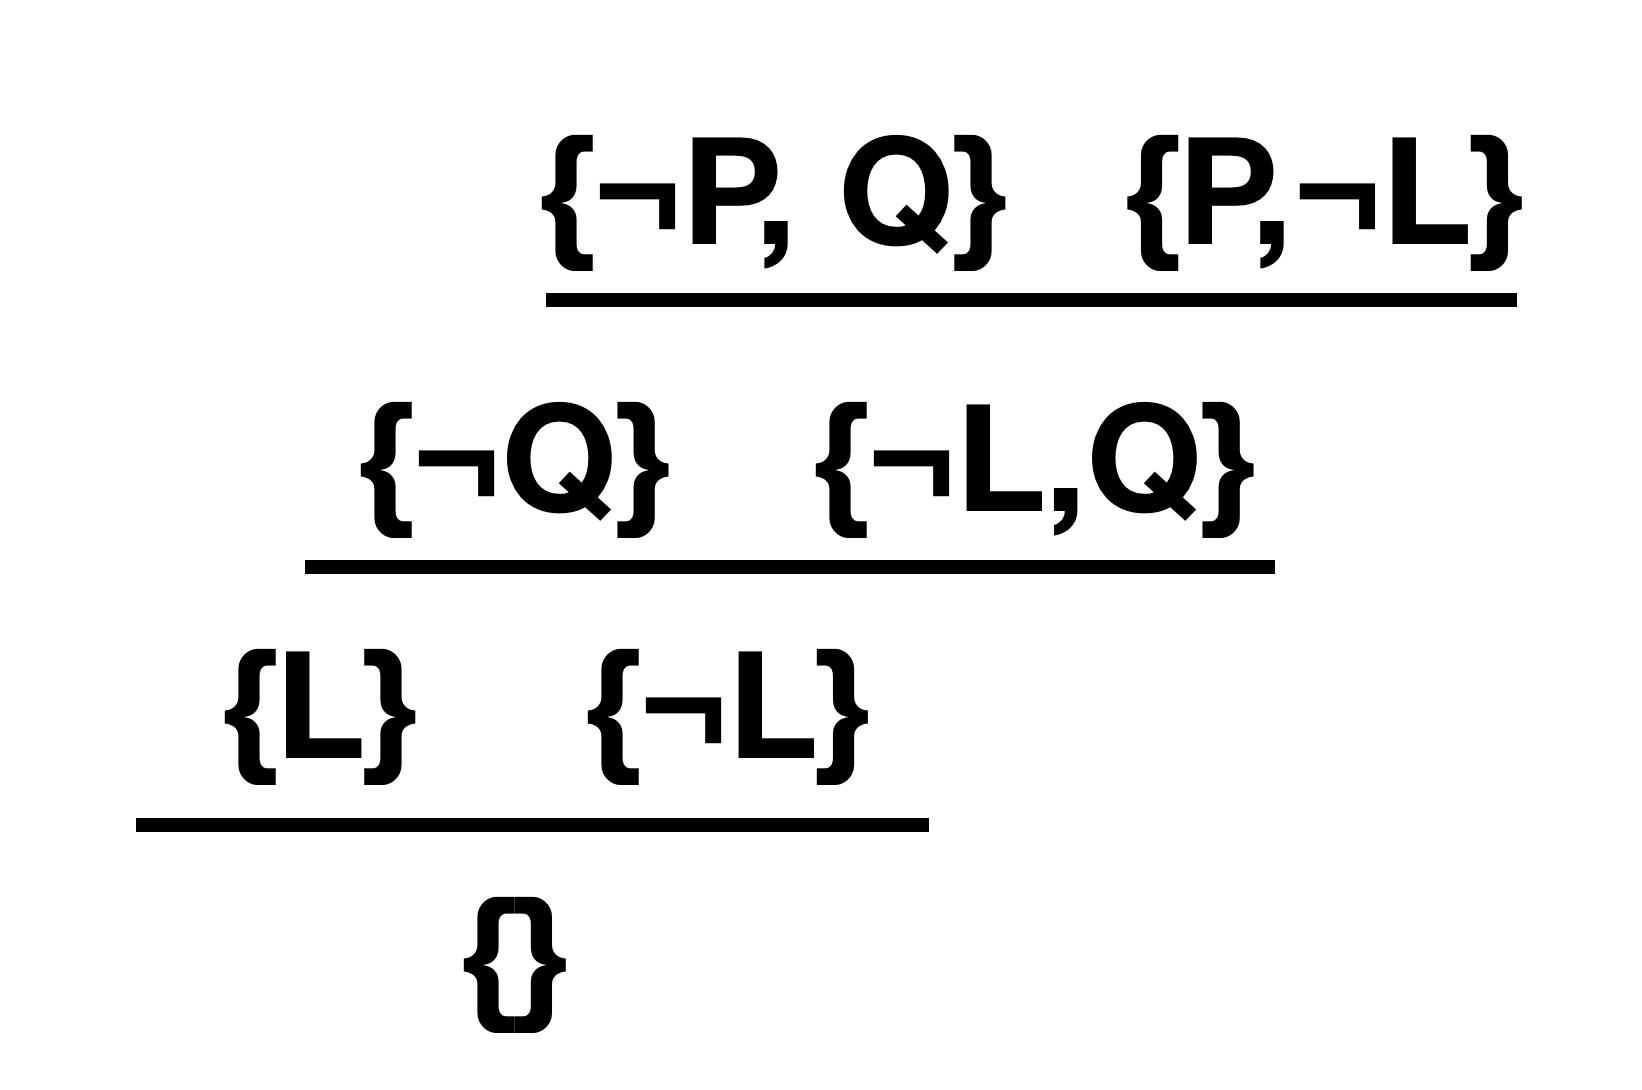
\includegraphics[scale=0.3]{images/res_expansion.png}}
\caption{Resolution steps shown in tree form}
\label{fig:res_expansion}
\end{figure}

\paragraph{Satisfiability of Resolution} We start by having two clauses $C_1=\lbrace L_1,...,L_n\rbrace$, $C_2=\lbrace P_1,...,P_m\rbrace$ and a literal that is the same in each clause but with a different sign $L_i=\neg P_j=K$, i.e. if $L_i$ is \textit{True} then $P_j$ is \textit{False}. We want to prove that $\lbrace C_1 \cup C_2 \rbrace \setminus \{K\}$ is satisfiable.\\
Suppose $C_1$ and $C_2$ are satisfiable, i.e. there exists a model $\mathcal{M}$; such that $\mathcal{M}\models C_1$ and $\mathcal{M}\models C_2$, and that $L_i$ is true in $\mathcal{M}$; it follows that $\neg L_1$ is \textit{False} in $\mathcal{M}$, thus $P_j$ is \textit{True} in $C_2$ and therefore $C_2$ must be \textit{True} in $\mathcal{M}$. Consequently, $C_1\cup C_2$ is true in $\mathcal{M}$. Since $\mathcal{M}$ is a model of $C_1,C_2$ by hypothesis, $C_1\cup C_2$  is true in M.\\
Same goes with $\mathcal{M}\models \neg L_i$.


\paragraph{Completeness of resolution}
\label{par:ground_res_theo}
We introduce the notion of \textbf{resolution closure} $RC(S)$ of a set of clauses $S$ that  is the set of all clauses derivable by repeated application of the resolution rule to clauses in $S$ or their derivatives.\\
It is easy to understand that $RC(S)$ is finite because there are only finitely many distinct clauses that can be constructed out of the symbols $P_1, . . . , P_k$ that appear in $S$ \footnote{This is true only if we are using the factoring step to remove duplicate literals.}.\\ 

Now let us consider the \textbf{ground resolution theorem} which states:
\textit{If a set of clauses is unsatisfiable, then the resolution closure of those clauses contains the empty clause}; that is :
\[S\quad unsatisfiable\quad iff\quad \{\}\in RC(S)\]
Now let's prove this the other way around, we want to prove that:
\[S\quad satisfiable\quad iff\quad \{\}\notin RC(S)\]
First we build a model of $RC(S)$ with the following procedure.\\ For $i$ in $range(k)$:
\begin{itemize}
\item Given a clause $C_k \in S$ that contains $\neg P_i \in C_k$ and all its other literals are set to \textit{False}: $C_k=false\vee...\vee false\vee \neg P_i$; assign $False$ to $P_i$, so to make $C_k$ true.
\item Otherwise assign \textit{True} to $P_i$.
\end{itemize}
So now we have a model of $S$. Since we must prove that $RC(S)$ is satisfiable, thus have some models, let's assume that what we just got is not a model, then we must have been wrong at some iteration $i$. That is setting the symbol $P_i$ causes some clause $C$ to becomes false, since we \textit{do not have a model} all the other clauses must be already false. So $C$ can be one of the following possibilities:
\begin{itemize}
\item $C=false\vee...\vee false\vee P_i$
\item $C=false\vee...\vee false\vee \neg P_i$
\end{itemize}
If \textit{only one} of the two is in $RC(S)$ then the algorithm would assign the right value to make $C$ true. So the only way to have $C$ false is that \textit{both} possibilities are in $RC(S)$, but this is impossible since $RC(S)$ is \textbf{closed under resolution}, that is the two possibilities would have been resolved by the algorithm.

\subsection{Chaining}
\label{subsec:chaining}


\subsubsection{Forward Chaining}

\paragraph{Definition}
Determines if a single proposition symbol $q$ \footnote{What is asked to the KB, i.e. the query.} is entailed by a KB of definite clauses \footnote{Definite clauses means the KB contains either facts (positive literals) or implication with an \textit{atomic} conclusion and, for premise, either an atom or a conjunction of literals. }. It begins from known facts in the knowledge base \footnote{For this reason it is called \textbf{data driven}.}. If all the premises of an implication are known, then its conclusion is added to the set of known facts. This process continues until the query $q$ is reached or until no further inferences can be made. The main point to remember is that it runs in linear time.

\paragraph{Example}
Given the following KB:
\begin{itemize}
\item $P \Rightarrow Q$, equal to $\neg P \vee Q$ (definite clause)
\item $L \wedge M \Rightarrow P$, equal to $\neg L \vee \neg M \vee P$ (definite clause)
\item $B \wedge L \Rightarrow M$, equal to $\neg B \vee \neg L \vee M$ (definite clause)
\item $A \wedge P \Rightarrow L$, equal to $\neg A \vee \neg P \vee L$ (definite clause)
\item $A \wedge B \Rightarrow L$, equal to $\neg A \vee \neg B \vee L$ (definite clause)
\item $A$, (known fact, since positive literal)
\item $B$, (known fact, since positive literal)
\end{itemize}
We query Q \footnote{That is we ask the KB about the truthfulness of Q.}.\\
 The KB can bee seen as an \textbf{AND-OR Graph} where the implications are $OR$ arches while the $\wedge$ are $AND$ arches (Figure \ref{fig:forward_graph_1}).\\


\begin{figure}[t]
\centering
\fbox{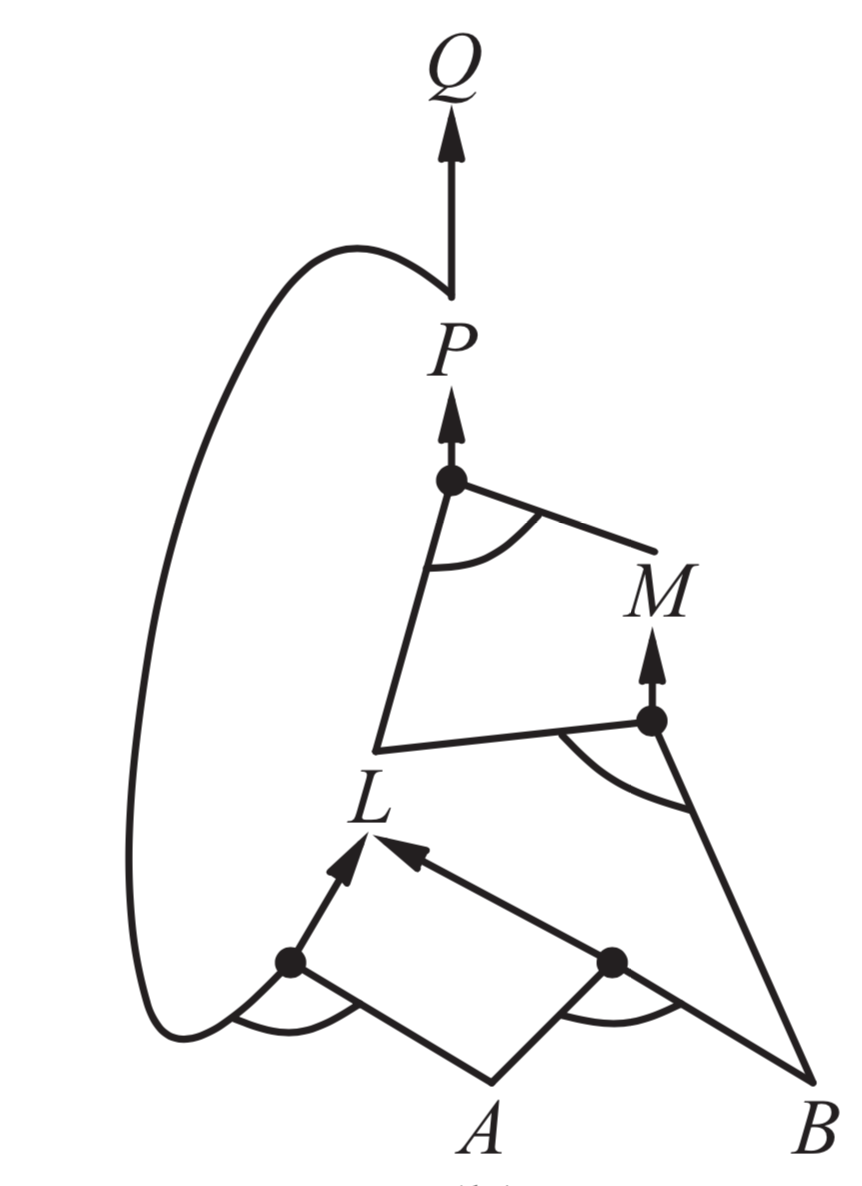
\includegraphics[scale=0.3]{images/forward_graph.png}}
\caption{AND-OR graph for definite clause KB}
\label{fig:forward_graph_1}
\end{figure}
The flow of the algorithm works as illustrated in Figure \ref{fig:forward_graph_2}.


\begin{figure}[H]
\centering
\fbox{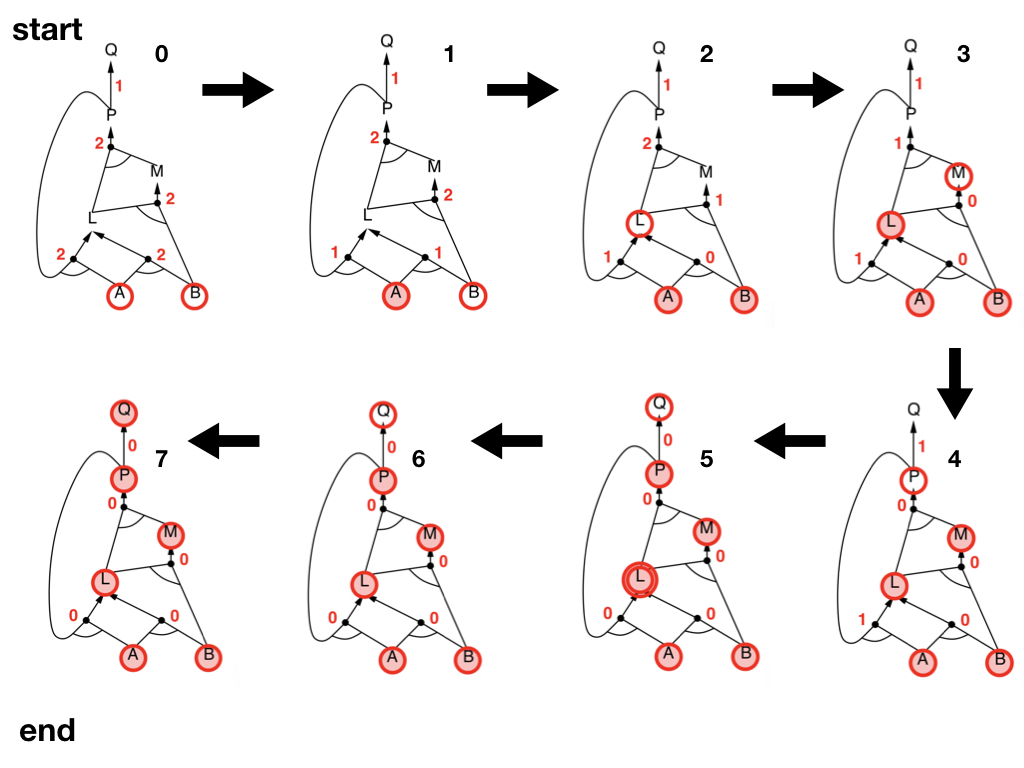
\includegraphics[scale=0.45]{images/forward_graph_2.jpeg}}
\caption{Forward Chaining for KB graph}
\label{fig:forward_graph_2}
\end{figure}


\paragraph{Proof}
We can affirm that the algorithm is \textbf{sound} since every step is an application of Modus Ponens.\\
For the \textbf{completeness} we need to prove that every possible atomic sentence can be derived from the KB. We first introduce the notion of \textbf{fixed point} which is a state of the algorithm in which no more inference can be done; then we consider to be in the final state $m$ that is a model \footnote{In which there has been various assignment of \textit{True/False} for the literals.} because we cannot apply Modus Ponens to any other clause.\\
Since the final state is in Horn form \footnote{As the whole KB.} we have a conjunction of disjunctions, so to be a model \footnote{True interpretation.} every clause must be \textit{True}. To prove this let's consider the opposite:
\begin{itemize}
\item Let's take a generic clause $C=a_1\wedge...\wedge a_n\Rightarrow b$ in $m$. This clause have a general number of conjunctions $n$ in its premise.
\item Suppose that $C$ is false in $m$.
\item For an implication to be \textit{False} we need the premise $a_1\wedge...\wedge a_n$ to be \textit{True} and the conclusion $b$ to be \textit{False}.
\item But if that is the case I would apply Modus Ponens again $\frac{a_1\wedge...\wedge a_n\Rightarrow b\quad a_1\wedge...\wedge a_n}{b}$ and conclude $b$ True, so in fact I'm not in a fixed point and this contradicts the assumption.
\end{itemize}


We can conclude, therefore, that the set of atomic sentences inferred at the fixed point defines a model of the original KB. Furthermore, any atomic sentence q that is entailed by the KB must be true in all its models and in this model in particular. Hence, every entailed atomic sentence q must be inferred by the algorithm.

\subsubsection{Backward Chaining}
On the other hand the backward chaining works its way from the query $q$ \footnote{Note that if the query is true the algorithm stops immediately.} and find those implication which conclusions are equal to $q$. If all the premises of a given implication which resolve in $q$ are true then we can conclude that $q$ is true itself.\\
This kind of reasoning is called \textbf{goal directed} reasoning and it usually works in linear size in respect to the size of the KB.



\subsection{Proposal for model checking}
\label{subsec:search_alg}
In this section, we describe two families of efficient algorithms for general propositional inference based on model checking: One approach based on backtracking search, and one on local hill-climbing search. Notice that these algorithms are used for checking the \textbf{satisfiability} (SAT) of a problem.

\subsubsection{DPPL}
Also known as David-Putnam, Logemann, Loveland algorithm, it takes as input a sentence in conjunctive normal form (Section \ref{subsec:cnf}) and uses a recursive depth-first enumeration of all possible interpretations. To speed up the algorithm we can introduce some improvements.

\paragraph{Early Termination} A clause is true if \textit{any} literal is true \footnote{Remember that a clause is a disjunction of literals of the form $C_1\vee C_2\vee...\vee C_n$.}, hence if we encounter a true literal in a clause we can stop looking at it and give it the value \textit{true} \footnote{Similarly a sentence (conjunction of clauses) is false if \textit{any} clause is false.}.\\
For example having $(A\vee B)\wedge(A \vee C)$, if $A$ is true then we do not need to look for the values of $B,C$.

\paragraph{Pure Symbol} is a symbol which always appears with the same "sign", i.e. negated or not, so it can be assigned a value once for all the clauses.
For example:
\[(A\vee\neg B)\wedge (\neg B \vee \neg C)\wedge(C \vee A)\]
In this case the literal A is a pure positive symbol, B is a pure negative while C is impure.

\paragraph{Unit clause} is a clause with only one literal. This can be either because
\begin{itemize}
\item We have a clause with just one literal (fact). Or
\item We have a clause with multiple literals that are false \footnote{Since clauses are disjunction, false literals can be removed if there are some other that can assume the value true.} except for this last one \footnote{This is also called \textbf{unit propagation}.}.
\end{itemize}

\paragraph{Component analysis} We can divide clauses into independent subset when they \textit{do not share} any common literal. By dividing them we can parallelize the job as well as prune large part of the state space 	\footnote{No necessity to check the constraint of a literal in other clauses which do not have it. }

\paragraph{Variable and Value ordering} A general rule is to always try the value \textit{true} before \textit{false}. While the \textbf{degree heuristic} suggests choosing the variable that appears most frequently over all remaining clauses \footnote{Everything we saw in the planning part of the course.}.

\paragraph{Intelligent Backtracking} Also discussed in the Planning part of the course, intelligent backtracking keeps tracks of conflicts \footnote{Literals that may create a conflict with other literals.} so to cut off useless searches steps.

\paragraph{Random restarts} When the algorithm gets stuck for a long time execute a restart from the root point.

\paragraph{Clever indexing} at implementation level.

\subsubsection{Local Search Algorithm}
These algorithms works by flipping the truth value of one symbol at a time. The search space usually contains many local minima, to escape from which various forms of randomness are required. 

\paragraph{GSAT} Missing

\paragraph{WALKSAT} 
The algorithm picks an unsatisfied clause and picks a symbol in the clause to flip. It chooses randomly between two ways to pick which symbol to flip: 
\begin{itemize}
\item A \textit{min-conflicts} step that minimizes the number of unsatisfied clauses in the new state.
\item A \textit{random walk} step that picks the symbol randomly.
\end{itemize}
This type of algorithm is very similar to simulate annealing studied in the Local search part.
WALKSAT may end with the following outcomes:
\begin{itemize}
\item A model; thus the input sentence is satisfiable.
\item A failure; then there are two possibilities:

	\begin{itemize}
	\item Either the sentence is unsatisfiable, or
	\item The algorithm needs more time to complete the search \footnote{Note that if there is no limit to the number of flips and the sentence is unsatisfiable then the algorithm may never end.}.
	\end{itemize}
\end{itemize}

\subsubsection{Random SAT problem}
Depending on the number of clauses $m$ and symbols $n$ we can either have an \textit{under-constraint} problem ($n>m$) or a \textit{over-constraint} problem ($m>n$) \footnote{Giving that each symbol may not appear twice in a clause and no clauses may appear twice in the sentence.}. Given the ration $r=m/n$, when the ratio approaches zero then the probability of the problem to be satisfiable approaches one and vice versa. As you can see from Figure \ref{fig:sat} around the value $r=m/n=4.3$ the probability for the sentence to be satisfiable approaches zero.


\begin{figure}[H]
\centering
\fbox{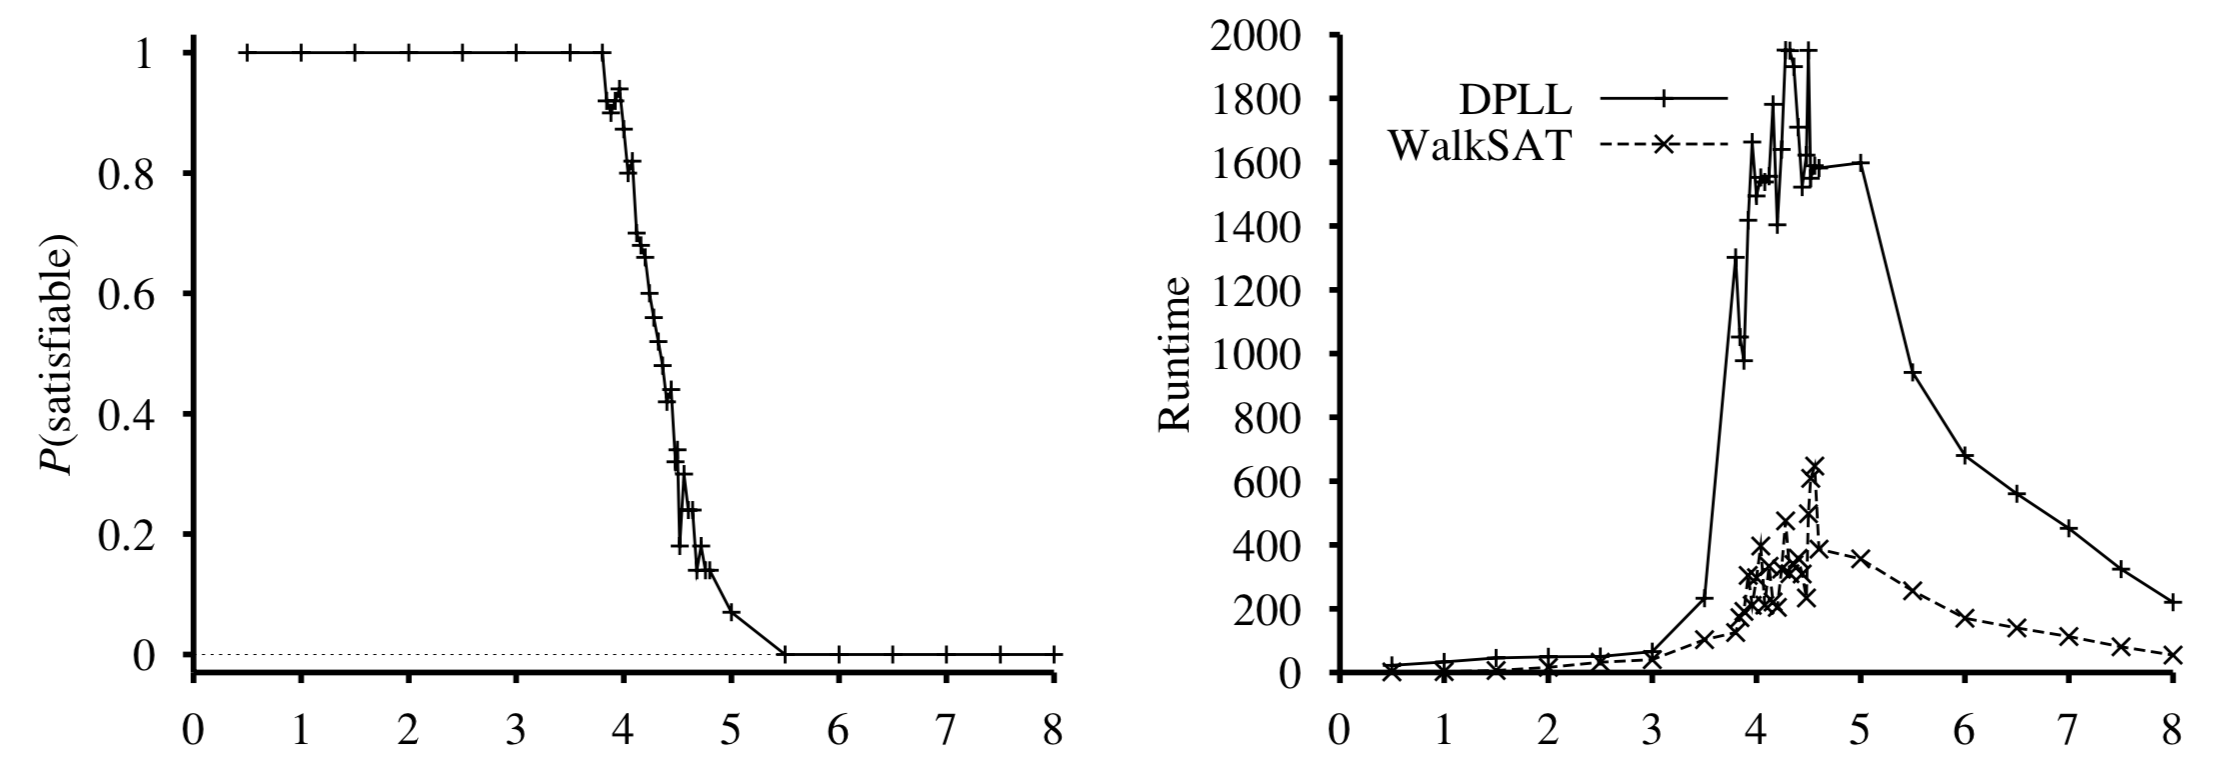
\includegraphics[scale=0.3]{images/sat.png}}
\caption{(Left) Graph showing the probability that a random  sentence with n = 50 symbols is satisfiable, as a function ratio m/n. (Right) Graph of the median run time on random sentences. The most difficult problems have a ratio of about 4.3.}
\label{fig:sat}
\end{figure}

\newpage
\section{First Order logic}

\subsection{Syntax and Semantic}

One of the most important proprieties about propositional logic that holds for First Order Logic (FOL from now on) is the \textbf{compositionality}, that is the meaning of a sentence is a function of the meaning of its parts. For example given $S_1=$\textit{I have don't want to write this} and $S_2=$\textit{I would love to watch Netflix} it would be weird if $S_1 \wedge S_2=$\textit{Tomorrow will be cold}.\\
Moreover propositional logic assumes that there are facts that either hold or do not hold in the world \footnote{Each fact can be in one of two states: true or false.}, while FOL assumes that the world consists of objects with certain relations among them that do or do not hold. Hence in both logic a sentence represents a fact and the agent either believes the sentence to be true, believes it to be false, or has no opinion. 

\paragraph{Structure}
FOL assumes the world contains:
\begin{itemize}
\item \textbf{Objects} like: pc, tv, beer....
\item \textbf{Relations} are sets of tuples of objects that are related. Depending on the number of tuple in the set we can have:
	\begin{itemize}
	\item \textit{Proprieties} (or unary relationship) that have just one tuple in the set; such as:\textit{red, round, big}...
	\item \textit{General} (or $n$-ary relationship)  which may have $n$ tuples; like:\textit{ bigger than, has color, owns}...
	\end{itemize}

\item \textbf{Functions}  For example: \textit{father of, best friend}...
\end{itemize}

\paragraph{Example}
Given the sentence \textit{"The next MidTerm will be easier then the first one"}\footnote{Probably not a model.} I have that:
\begin{itemize}
\item \textit{Objects}: Midterm, one
\item \textit{Proprieties}: next, first (unary)
\item \textit{Functions}: easier than
\end{itemize}


\paragraph{Symbols} For each one on the structures we have a related symbol:
\begin{itemize}
\item \textbf{Constants}: stands for objects.
\item \textbf{Predicates}: stands for relations.
\item \textbf{Functions}: stands for functions \footnote{You don't say.}
\end{itemize}
The last two comes with an \textbf{arity} that is the number of arguments they are referring to \footnote{For example the function \textit{Sibling(x,y)} has arity 2 (since we need a subject and a brother), while the function \textit{Human(x)} has arity 1.}.

\paragraph{Interpretation vs Model}
A model in first-order logic consists of a set of objects and an interpretation that maps constant symbols to objects, predicate symbols to relations on those objects, and function symbols to functions on those objects.\\
Given a domain $\mathcal{D}$, an interpretation is a function $\mathcal{I}$ which maps:
\begin{itemize}
\item Every constant symbol $c$ into an element of $\mathcal{D}$.
\item Every $n$-ary\footnote{A function with $n$ arguments.} function symbol $f$ into a  function $f^I$: $\mathcal{D}^n\rightarrow \mathcal{D}$. More specifically $f$ is a function which may assume any value in the domain $\mathcal{D}^n$, while $f^I$ assumes just one ($\mathcal{D}$).
\item Every predicate symbol $P$ into a  $n$-ary relation $P^I$: $P^I\subset \mathcal{D}^n$. This means that a predicate symbol, e.g. ????????????????
\end{itemize}

\paragraph{Terms}
are a logical expressions that refers to an object. That is what is used to refer to a particular object in the domain; they can be:
\begin{itemize}
\item \textbf{Constants} symbols; for example the color red, or that guy Eric over there.
\item \textbf{Functional} terms; which are functions applied to constant symbols such as: \textit{BestFriendOf(Eric)} or \textit{Mother(Marta)}.
\end{itemize}
Notice that both refer to an "object" in the domain, one directly (constants), while the other indirectly. A functional term can be used both for not known constants, like the name of Marta's mother, but they can also be used for thing we do not bother to name, e.g. \textit{LeftArmOf(Edoardo)}. 

\paragraph{Atomic Formulas}
An atomic formula (or atom for short) is a predicate symbol with a number $n\in [0,\infty]$ of terms. For example given $t_1,...,t_n$ terms, the following are all atoms:
\begin{itemize}
\item \textit{Sibling($t_i,t_j$)}:  predicate symbol with arity 2.
\item $Friend(t_1,...,t_n)$: predicate symbol with arity $n$.
\item $t_i=t_j$: predicate symbol $=$ with arity 2, can be written as $Equals(t_i,t_j)$
\item $ParentOf(ParentOf(x))$ is the grandparent of $x$ and has arity 1.
\item $\bot ,\top$ are atoms.
\end{itemize}

\paragraph{Terms vs Atoms}
So what is the difference between this two symbols?\\
The difference is in the use of relationships, for example:
\begin{itemize}
\item \textit{BatCave, CaveOf(Batman)} are terms, while \textit{Big(BatCave),Big(CaveOf(Batman))} are atoms.
\item Equal symbols generate atoms, for example \textit{MobileOf(Batman)} and \textit{BatMobile} are terms, where \textit{MobileOf(Batman)=BatMobile} is an atom.
\end{itemize}
Moreover a term is called \textbf{ground} if it does not contain variables \footnote{Later explained}, like \textit{CaveOf(Batman)}.

\paragraph{Complex Sentences}
When we have atoms joint by some logic connectives then we call them \textbf{complex sentence}, for example:
\begin{itemize}
\item $\neg Friends(Superman,LexLutor)$
\item $Superman\wedge Kryponite \Rightarrow Weak(Superman)$
\end{itemize}


\paragraph{Equality}
The equations symbol $=$ is used to indicate that two terms refer to the same object \footnote{Can be used to state fact about the world.}, while the negation symbol $\neq$  is used otherwise.


\paragraph{Database Semantics}
\label{sec:database_semantic}
\begin{itemize}
\item \textbf{Unique name assumption}: every constant symbol refers to a distinct object.
\item \textbf{Close-world assumption}: atomic sentences not known to be true are false.
\item \textbf{Domain closure}: each model contains no more domain elements than those named by the constant symbols.
\end{itemize}

\subsubsection{Quantifiers}
\label{sec:quantifiers}
We first introduce the concept of \textbf{variables} \footnote{Variables will be in lowercase.} that are equals to terms, thus can be used as arguments for functions.
Moreover a \textbf{free} variable is one that is not in the scope of any quantifier, elsewhere the variable is called \textbf{bounded}.\\ 
Then we have to talk about \textbf{extended interpretations} that specifies a domain \footnote{The domain is the set of individual objects.} element for which a variable exists

\paragraph{Universal Quantifier}
If we consider the sentence \textit{Every guy literally only want one thing} \footnote{And it's fucking disgusting!}, instead of enumerating every possible guy we can use:
\[\forall x\quad Guy(x)\Rightarrow WantOneThing(x)\]
that is translated in:\\
\begin{center}
For all $x$, if $x$ is a guy, then $x$ wants one thing.

\end{center}




\subparagraph{Implication vs Conjunction}
The question that arises is why do we have to use implication in the universal quantifier and not a conjunction?\\

Consider the following example:
\begin{itemize}
\item \textit{A(X)= is an apple}.
\item \textit{D(X)= is delicious}.
\end{itemize}

We want to consider an universe $U$ in which $all$ the apples are delicious, i.e. if the object is an apple then it is delicious, we must write:
\[\forall x\in U,\ A(x)\Rightarrow D(x)\]
That means for all objects in the universe, if $x$ is an apple $A(x)$, then $x$ is delicious $D(x)$. If we take a look at the truth table (Figure \ref{fig:truth_table}) we notice that the implication is has three rows in which is $True$, for every $x$:
\begin{enumerate}
\item If it is an apple and it is delicious.
\item If it is not an apple and it is delicious.
\item If it is not an apple and it is not delicious.
\end{enumerate}
This means that if we have an avocado as $x$ then the above formula will be true. So why is this?
The important thing to understand is that we only care about an universe in which $all$ apples are delicious, i.e. there can not be any non-delicious apple \footnote{First line of the truth table.}, nothing matters when it comes down to avocado. So the fact than an implication becomes vacuously for non-apple object is not in our scope of interest.\\
On the other hand, if we want to exclude the other two possibilities (2,3), we are saying that \textit{"any fruit is an apple and is delicious"}\footnote{Overly strong statement.}, hence \textit{all fruits are delicious apples}:
\[\forall x\in U,\ A(x) \wedge D(x)\]

\paragraph{Existential Quantifier}
On the other hand, if we do not want to specify a propriety for each object of a domain, but either we want to say that it exists \textit{at least one} object with a certain propriety we use the \textbf{existential quantifier}, e.g. \textit{Some student will pass the midterm}:
\[\exists x\quad Student(x) \wedge Pass(x)\]
Which is read as:
\begin{center}
There exists some $x$ such that $x$ is a student and $x$ will pass the Midterm (hopefully).
\end{center} 


\subparagraph{Conjunction vs Implication}
Same as before the question is : \textit{why do we use conjunction for existential quantifier}?\\
Like previously said, the conjunction for an universal quantifier makes the formula overly strong \footnote{All objects are delicious apples}, while the use of the implication for the existential quantifiers makes the formula overly week.\\
Going back to the apple example, we want to say that there are some apples which are delicious, if we use the implication symbol then the formula will return $True$ as soon as there is an object which is either a delicious non-apple or a non-delicious non-apple, so the look for some delicious apple stops immediately.\\
It is useful to imagine the existential quantifier to be like a disjunction in which as soon as we encounter a $True$ element we can stop the look for other and just return $True$.
On the other hand the implication needs to look for all the objects since its behavior is closer to the one of a conjunction.

\paragraph{Nested Quantifiers}
We can use multiple quantifiers in the same formula to express different kind of proprieties. For example, given the function $Love(x,y)$ that can be read as, $x$ loves $y$, we can say the following things:
\begin{itemize}
\item Everybody loves somebody:
\[\forall x \exists y Loves(x,y)\]
\item Somebody loves us
\[\forall x \exists y Loves(y,x)\]
\item X loves everybody
\[\exists x \forall y Loves(x,y)\]
\item Everybody loves x
\[\exists x \forall y Loves(y,x)\]
\end{itemize}


\paragraph{Connection between $\forall$ and $\exists$}
Saying that \textit{everyone likes professor Nardi} is like saying that \textit{there is no one who dislikes him}. 
So we can make use of this information to switch between universal and existential quantifiers as shown in Table \ref{tab:quant_equiv}.

\begin{table}[H]
\centering
\setlength\extrarowheight{5pt}

    \begin{tabular}{|l|l|}
        \hline
		Quantifiers & Equivalences\\ \hline\hline
        \forall x\ \neg P \equiv \neg \exists x\ P  & \neg(P\vee Q) \equiv \neg P \wedge \neg Q \\ \hline
        \neg \forall x\ P \equiv \exists x\  \neg P & \neg(P\wedge Q) \equiv \neg P \vee \neg Q \\ \hline
        \forall x\ P \equiv \neg \exists x\ \neg P  & P \wedge Q \equiv \ned(\ned P\vee\neg Q)  \\ \hline
        \exists x\ P \equiv \neg \forall x\ \neg P  & P\vee Q \equiv \neg(\neg P\wedge\neg Q)  \\\hline
        \forall x\ (P_1 \vee P_2) \equiv  \forall x\ P_1 \vee P_2   & if x \notin var(P_2) \\\hline
        \exists x\ (P_1 \wedge P_2) \equiv  \exists x\ P_1 \wedge P_2   & if x \notin var(P_2) \\\hline
        \forall xP(x)\equiv \forall y P(y) & \exists xP(x)\equiv \exists y P(y) \\\hline
        \forall x\forall y P(x,y) \equiv  \forall y\forall x P(x,y) \equiv  \forall x, y P(x,y) &
        \exists x\exists y P(x,y) \equiv  \exists y\exists x P(x,y) \equiv  \exists x, y P(x,y)\\\hline
        \forall x P(y) \equiv P(y) &\exists x P(y) \equiv P(y)\\\hline
        (\forall x P_1)\Rightarrow P_2 \equiv \exists x(P_1\Rightarrow P_2) & x not free in P_2\\\hline
        (\exists x P_1)\Rightarrow P_2 \equiv \forall x(P_1\Rightarrow P_2) & x not free in P_2\\\hline
        P_2\Rightarrow \forall x P_1 \equiv \forall x(P_2\Rightarrow P_1) & x not free in P_2\\\hline
        P_2\Rightarrow \exists x P_1 \equiv \exists x(P_2\Rightarrow P_1) & x not free in P_2\\\hline
    \end{tabular}
\caption{Quantifiers equivalences}
\label{tab:quant_equiv}
\end{table}

\subsection{Using First Order Logic}
Sentences which are added to the KB using \textit{TELL} are called \textbf{assertion} that states some truth about the world. On the other hand, queries are information \textit{ASK}ed to the KB, if they are logically entailed by the KB they should be answered positively. Similarly the \textit{AskVars} action ask the KB for the values of the formula that make it true, such answers are called substitutions (Section \ref{subsec:prop_vs_fol}) \footnote{Usually reserved for KB of only Horn Clauses.}.\\
Depending on the type of knowledge the KB is made out of we may have:
 \begin{itemize}
\item \textbf{Intentional Knowledge}: which are general laws about the domain, such as $\forall x,y\  Mother(x,y) \Leftrightarrow Famale(x)\wedge Parent(x,y)$.
\item \textbf{Extensional Knowledge}: facts about a specific instance, like $Parent(Marco,Ugo)$. 
 \end{itemize}

\paragraph{FOL formulas}
In FOL formulas follows this rules, given the formulas $A,B$:
\begin{itemize}
\item Every atom is a formula.
\item $\neg A$ is a formula.
\item If $\circ$ is a binary operator, then $A\circ B$ is a formula.
\item Given a variable $x$, $\forall x\ A$ and $\exists x\ A$ are formulas.
\end{itemize}

\subsection{Truth, Interpretation and Models}

\newcommand{\satisfy}{\textcolor{red}{\models}} 
\newcommand{\nsatisfy}{\textcolor{red}{\nvDash}} 

Remember that a \textit{closed formula}, also called a sentence, is a formula without free variables. So given a sentence $\phi$ and a structure $\mathcal{U}=\langle D, I \rangle$ we denote the truth of $\phi$ as:
\[\mathcal{U} \satisfy \phi\]
Meaning that the $\mathcal{U}$ satisfies \footnote{Note that in this case $\satisfy$ is read satisfies and it is red.} $\phi$ if $\phi$ is true in the $\mathcal{U}$. The following cases are used for satisfiability:
\begin{itemize}
\item $\mathcal{U}\satisfy \top$ and $\mathcal{U} \nsatisfy \bot$
\item If $A$ is a closed formula $P(t_1,...,t_n)$ then
\[\mathcal{U} \satisfy A\quad iff\quad \langle t_1^I,...,t_n^I\rangle \in P^I\]
\item $\mathcal{U} \satisfy \neg A$ iff $\mathcal{U} \nsatisfy A$
\item $\mathcal{U} \satisfy A \wedge B$ iff $(\mathcal{U} \satisfy A)\wedge \mathcal{U} \satisfy B$
\item $\mathcal{U} \satisfy (A \Rightarrow B)$ iff $(\mathcal{U} \satisfy A)\Rightarrow (\mathcal{U} \satisfy B)$
\item $\mathcal{U} \satisfy (A \leftrightarrow B)$ iff $(\mathcal{U} \satisfy A)\wedge (\mathcal{U} \satisfy B)$ or $(\mathcal{U} \nsatisfy A)\wedge (\mathcal{U} \nsatisfy B)$
\item $\mathcal{U} \satisfy \forall x\ A$ iff $\forall d \in D, \mathcal{U}\satisfy \lbrace d \rightarrow x\rbrace$
\item $\mathcal{U} \satisfy \exists x\ A$ iff $\exists d \in D, \mathcal{U}\satisfy \lbrace d \rightarrow x\rbrace$
\end{itemize}

For what regard models we have that if $\mathcal{U} \satisfy A$ then $\mathcal{U}$ is a \textbf{model} of $A$ \footnote{$A$ is true in $\mathcal{U}$.}.

\paragraph{Validity and satisfiability}

We have that if a formula $A\in \mathcal{L}$ is true in every structure of a language $\mathcal{L}$, then $A$ is \textbf{valid}.\\
On the other hand, given a set of formulas $\Gamma$, if there exists a structure $\mathcal{U}$ such that $\mathcal{U} \satisfy A$ for every $A \in \Gamma$ then $\Gamma$ is \textbf{satisfiable}, mathematically:
\[\Gamma = \lbrace A_1,...,A_n \rbrace,\ iff\ \exists\ \mathcal{U} :\mathcal{U}\satisfy A_i, \forall A_i \in Gamma\ \Rightarrow \Gamma\ satisfiable\]
We can derive the notion of \textbf{logic entailment} $\gamma \models A$, where $A$ is a closed formula, form the satisfiability, in the following way:\\
For every structure $\mathcal{U}$ of the language $\mathcal{L}$, $\forall B\in \Gamma:\mathcal{U} \satisfy B$, we have $\mathcal{U} \satisfy A$ then  $\gamma \models A$.


\subsection{Propositional vs First Order Logic}
\label{subsec:prop_vs_fol}

\newcommand{\subst}[1]{Subst(\theta,#1)} 

First-order inference can be done by converting the KB to propositional logic and using propositional inference. This can be done by replacing the quantifiers as explained in the following paragraphs.

\subsubsection{Universal instantiation}
\label{subsubsec:UI}

\textbf{UI} for short, is used for the universal quantifier and it says that we can substitute a variable with a ground term \footnote{Term without variables.} to infer the sentence.\\
The \textbf{substitution} is written an follow:
\[Subst(\theta,\alpha)=\frac{\forall v\ \alpha}{Subst(\lbrace v/g\rbrace,\alpha)}\]
where $\theta$ is the substitution applied to the term $\alpha$ for any variable $v$ and ground term $g$. \\
The UI can be applied many times to produce multiple consequences that will be added to the KB  preserving its logical equivalence.

\paragraph{An Example}
Given the formula:
\[\forall x,y\quad Loves(x,y)\]
We can substitution like this:
\[Subst(\lbrace x/Anna,y/Enrico \rbrace,Loves(x,y))=Loves(Anna,Enrico)\]
\textit{And} like this:
\[Subst(\lbrace x/Enrico,y/Anna \rbrace,Loves(x,y))=Loves(Enrico,Anna)\]

\subsubsection{Existential instantiation}
\label{subsubsec:EI}
\textbf{EI} for short, in this case the variable is replace with \textit{a single} constant symbol $C$ that \textbf{does not} appear in the KB. The idea is saying that there is an object $C$ that satisfy the existential quantifier, but we are not specifying which is it.\\
After applying EI we need to remove the existential quantifier \footnote{Skolemization.} and our new KB will \textit{not} be logically equivalent to the old one, but it can be shown that it is satisfiable exactly when the original KB is satisfiable.

\paragraph{An Example}
Given the formula:
\[\exists x\ Game(x)\wedge PlayOnPc(x,Nicolo)\]
We have \textit{the only} substitution:
\[Game(G_1)\wedge PlayOnPc(G_1,Nicolo)\]
Where $G_1$ is a generic constant symbol referring to some cool game I want to play.


\subsubsection{Propositionalization}
Is the technique of reducing first-order inference to propositional inference. The problem is that with function symbols we may have an infinite domain \footnote{For example \textit{Father(Father(Father(Father(Jhon)))).}}, so how can we preserve the entailment?\\
Thanks to Jacques Herbrand (1930) we have a theorem which states the following:
\textit{if a sentence is entailed by the original, first-order KB, then there is a proof involving just a finite subset of the propositionalized KB}. The problem with propositionalization is that it generates a lot of irrelevant sentences, with $p$  predicates of $k-$arity and $n$ constants we have $p\cdot n^k$ instantiations.\\
The question of entailment for first-order logic is \textit{semidecidable}, that is, algorithms exist that say yes to every entailed sentence, but no algorithm exists that also says no to every non-entailed sentence
 
\paragraph{An Example}
Given the following KB:
\[\forall x\  Student(x) \wedge Stressed(x) \Rightarrow StudyingAI(x)\]
\[Student(Edoardo),Student(Marco), Professor(Nardi)\]
We ca use UI to have:
\[Student(Edoardo) \wedge Stressed(Edoardo) \Rightarrow StudyingAI(Edoardo)\]
\[Student(Marco) \wedge Stressed(Marco) \Rightarrow StudyingAI(Marco)\]
\[Student(Edoardo),Student(Marco), Professor(Nardi)\]
So that the new propositionalized KB is:
\[Student(Edoardo), Stressed(Edoardo), StudyingAI(Edoardo),Student(Marco),\]
\[Stressed(Marco), StudyingAI(Marco), Professor(Nardi)\]

\paragraph{Horn Clauses}
We can have the following for every element of the FOL:
\begin{itemize}
\item \textit{Facts}: $\top\RightarrowA(x)$ ($A(x)$ for simplicity). 
\item \textit{Rules}: $A_1(x)\wedge...\wedge A_n(x)\Rightarrow B(x)$
\item \textit{Goals}: $A_1(x)\wedge...\wedge A_n(x)\Rightarrow \bot$ \footnote{We are using $\bot$ since want to prove the falsity of the premise is impossible so the premise is true.}
\end{itemize}


\subsubsection{Generalized Modus Ponens}

When we have an implication of the kind:
\[p_1 \wedge ... \wedge p_n \Rightarrow q\]
If there is a substitution $\theta$ which makes every conjunct of the premises identical to a sentence in the KB, then we can infer $q$.\\
The \textbf{Generalized Modus Ponens} [GMP] works in the following way: given $n$ atomic sentences $p_1,...,p_n$ which are the premises of an implication $p_1\wedge ... \wedge p_n\Rightarrow q$, and given $n$ atomic sentences already in the KB $p_1',...,p_n'$ so that $Subst(\theta,p_i)=Subst(\theta,p_i')$ \footnote{This is that given the substitution $\theta$ we can transform a sentence $p$ into a known sentence $p'$ in the KB.} for all $i$, we can use \textit{GMP}:
\[\frac{p_1',...,p_n',\quad (p_1\wedge ... \wedge p_n\Rightarrow q)}{Subst(\theta,q)}\]
And infer a valid substitution for the query $q$.\\

\paragraph{Example}
Given a KB with the following information:
\begin{enumerate}
\item $\forall y\ Tired(y)$, everyone \footnote{Actually every object.} in the domain is tired.
\item $\forall x\ Student(x)\wedge Stressed(x) \wedge Tired(x) \Rightarrow NeedCoffe(x)$
\item $Student(Edoardo),Student(Luca), Stressed(Luca)$
\end{enumerate}

Considering the second line of the KB, we have that:
\begin{itemize}
\item $p_1=Tired(x)$
\item $p_2=Student(x)$
\item $p_3=Stressed(x)$
\item $q=NeedCoffe(x)$
\end{itemize}

So now we need a substitution $\theta$ such that $Subst(\theta,p')=Subst(\theta,p)$. Trying with:
\[\theta=\lbrace x/Edoardo, y/Edoardo \rbrace\]
Will not work since the KB has no notion about $Stressed(Edoardo)$ \footnote{Since the first line of the KB, implies that every one in the domain is tired the formula $Tired(x)$ will always be true. }. On the other hand, Luca is pretty stressed so we can use:
\[\theta=\lbrace x/Luca, y/Luca \rbrace\]
So we can conclude that $Subst(\theta, q)\longrightarrow Luca$.\\



\paragraph{Soundness}
It is easy to prove that the \textit{GMP} is sound since we need to prove that: given a sentence $p$ and a substitution $\theta$, we have:
\[p \models Subst(\theta,p)\] 
But this holds since it exactly what we have using \textit{UI}.

\subsubsection{Unification}
As before mentioned we need to find a substitution such that different logical expression looks identical ($\subst{p}=\subst{p'}$). We can use the \textbf{Unification} process that takes as input two sentences and returns an unifier for them\footnote{If exists.}:
\[Unify(p,q)=\theta\ \subst{p}=\subst{q}\]
We can have problems when having variables with the same name \footnote{As you will see in the next example.}, so we need to use a technique called \textbf{standardizing apart} which changes one of the two sentence's variables to avoid name clashes.\\
Finally we can say that, for every unifiable pair of expressions, there is a single \textbf{most general unifier} that is unique up to renaming and substitution of variables, for example $P(A,B)$ is less general than $P(A,x)$ that is less general than $P(y,x)$. 

\paragraph{Example}
Given the following KB:
\begin{enumerate}
\item $Knows(Homer, Marge)$, Homer knows Marge.
\item $\forall y\ Knows(y,Bart)$, everyone knows Bart.
\item $\forall y\ Knows(y,Mother(y))$, everyone knows their mother.
\item $\forall x\ Knows(x,Lisa)$, everyone knows Lisa.
\item $\forall y,z\ Knows(y,z)$, everyone knows everyone.
\end{enumerate}

We ask the KB which are the persons that $Homer$ knows: $q=AskVars(Knows( Homer,x))$. So we will have the following:
\begin{enumerate}
\item $Unify(Knows( Homer,x),Knows(Homer, Marge)=\lbrace x/Marge \rbrace$
\item $Unify(Knows( Homer,x),Knows(y, Bart)=\lbrace x/Bart, y/Homer \rbrace$
\item $Unify(Knows( Homer,x),Knows(y, Mother(y))=\lbrace y/Homer, x/Mother(y) \rbrace$
\item $Unify(Knows( Homer,x),Knows(x, Lisa)=Fail$, because the variable $x$ cannot be both $Homer$ and $Lisa$ at the same time \footnote{It should follow the behavior of point 2.}, so we use \textbf{standardizing apart}.
\item $Unify(Knows( Homer,x),Knows(y, z)$, returns two substitutions:
	\begin{enumerate}
	\item $\theta=\lbrace y/Homer, x/z \rbrace$, which is the \textbf{most general unifier}.
	\item $\theta=\lbrace y/Homer, x/Homer, z/Homer \rbrace$, which may be generated by the previous substitution with $\lbrace z/Homer \rbrace$.
	\end{enumerate}
\end{enumerate}



\subsection{Chaining}
Consider the following problem:
\begin{center}
\begin{textit}
The law says that it is a crime for an American to sell kinder eggs to hostile nations. The Easter Island, an enemy of America, has some kinder eggs, and all of its kinder eggs were sold to it by Roger Rabbit, who is American.

\end{textit}
\end{center}
We want to prove that Roger Rabbit is a criminal. First we need to convert the problem to a first-order definite clause KB:
\begin{enumerate}
\item "...it is a crime for an American to sell kinder eggs to hostile nations" results in:
\[American(x)\wedge KinderEgg(y)\wedge Sells(x,y,z)\wedge Hostile(z)\Rightarrow Criminal(x)\] \footnote{From now on we will not write the $\forall x,y,z$ symbol. Note that this kind of KB is called \textbf{Datalog}.}

\item "The Easter Island...has some kinder eggs", the sentence can be written as an existential formula of the form:
\[\exists x\ Owns(EasterIsland,x)\wedge KinderEgg(x)\]
We can use \textit{EI} \ref{subsubsec:EI} to remove the existential quantifier by adding some new constant $K_1$ resulting in:
\[Owns(EsterIsland,K_1),\quad KinderEgg(K_1)\]

\item "... all of its kinder eggs were sold to it by Roger Rabbit":
\[KinderEgg(x)\wedge Owns(EsterIsland,x)\Rightarrow Sells(RogerRabbit,x,EsterIsland)\]

\item We must know that an hostile object is an enemy of America:
\[Enemy(x,America)\Rightarrow Hostile(x)\]

\item "Roger Rabbit is American":
\[American(RogerRabbit)\]


\item "The Easter Island, an enemy of America":
\[Enemy(EsterIsland,America)\]
\end{enumerate}

\subsubsection{Forward Chaining}
Starting from the known facts, the algorithm triggers all the rules whose premises are satisfied, adding their conclusions to the known facts. The process repeats until the query is answered or no new facts are added. Notice that a fact is not new if it is just a \textbf{renaming} of a known fact \footnote{For example \textit{Likes(x,ice-scream)} and \textit{Likes(y,ice-scream)} are renaming of each other with the same meaning (everybody likes ice-scream).}.
The steps for the forward chaining are the following:
\begin{itemize}
\item Rule 3 is satisfied with $\subst{x}=\lbrace x/K_1 \rbrace$, so that $Sells(RogerRabbit,K_1,EsterIsland)$ is added to the KB.
\item Rule 4 is satisfied by $\subst{x}=\lbrace x/EsterIsland \rbrace$, so that $Hostile(EsterIsland)$ is added.
\item Finally rule 1 is satisfied with $\subst{x,y,z}=\lbrace x/RogerRabbit, y/K_1, z/EsterIsland \rbrace$ so we can add $Criminal(RogerRabbit)$.\\

Notice that we reached a \textbf{fixed point} in which no more inferences can be induced, but the difference with the propositional fixed point is that we may have universally quantified atomic sentence.\\
Moreover the algorithm is \textbf{sound} since every step is an application on \textit{GMP} and complete for definite clause knowledge bases; that is, it answers every query whose answers are entailed by any knowledge base of definite clauses.\\ Finally let $k$ be the maximum arity (number of arguments) of any predicate, $p$ be the number of predicates, and $n$ be the number of constant symbols. Clearly, there can be no more than $pn^k$ distinct ground facts, so after this many iterations the algorithm must have reached a fixed point.

\paragraph{Efficiency}
The previous mentioned process may be improved with :
\begin{itemize}
\item \textbf{Conjunction ordering}: the problem of finding an ordering to solve the conjuncts of the rule premise so that the total cost is minimized. It arises when we have many facts in the KB that need to be matched against a premise.\\
Given the rule 3 we have to find objects which are both  $KinderEggs$  owned by $EsterIsland$; so we must iterate through all the $n$ $KinderEggs$ and all the $m$ objects owned by $EsterIsland$. It is logical that if $n\ll m$ it will be faster to find the $KinderEggs$ first and then the object owned by $EsterIsland$.\\ This problem is exactly as the CSP-problem studied before \footnote{We can use the studied techniques such as \textit{minimum-remaining-value}...}, thus being NP-Hard.

\item \textbf{Incremental Forward Checking}: another problem is the one of matching redundant rules. It can be avoided if we consider that a rule is \textit{"new"} at iteration $t$ if it has been inferred by some facts generated in the previous iteration $t-1$, otherwise it would have been generated earlier.\\ Another problem is given by \textbf{partial matching} rules which are generated and discarded as soon as some atoms in the premise do not hold. Instead of discarding them we could leave them semi-generated and gradually complete them as new facts arrives.

\item \textbf{Irrelevant Facts}: finally, the algorithm does not distinguish between relevant and irrelevant facts. To address this issue we can either use backward chaining or deductive databases that uses forward chaining as the standard inference rule.
\end{itemize}

\subsubsection{Backward Chaining}
The backward chaining is a kind of AND/OR search, the $OR$ part because the goal query can be proved by any rule in the knowledge base, and the $AND$ part because all the conjuncts in a list of clauses must be proved.\\ It is a depth-first search so it suffers from problem such as repeated states and incompleteness.\\ It is the base for \textbf{Logic programming [PROLOG]} 

\newpage
\section{Resolution in First Order Logic}
For applying resolution we need to convert a sentence in \textit{Conjunctive Normal Form} CNF \footnote{Section \ref{subsec:cnf}.}, fortunately every sentence in FOL can be converted into an inferentially equivalent sentence in CNF; the difference between propositional CNF and FOL CNF is the presence of the existential quantifier.


\subsection{Skolem Normal Form}
\label{sec:skolemNF}
When removing existential quantifiers using $EI$ (Section \ref{subsubsec:EI}) we are assuming there exist an element, which we do not know, that satisfy the existential property.\\
Now consider the sentence \textit{"Everyone has a heart"}, that is translated in FOL with:
\[\forall x [Person(x)\Rightarrow \exists y\ Heart(y)\wedge Has(x,y)]\]
If we use $EI$ on thi s we obtain:
\[\forall x [Person(x)\Rightarrow  Heart(H)\wedge Has(x,H)]\]
The meaning of the sentence becomes \textit{"Everyone has the heart H"}, which is not the same as before since we make no distinction between hearts.\\
For this kind of problem we need a function which takes as input a person and returns the person's heart. Let us denote this function as $F(x)$ \footnote{Note that this function must not appear in the KB, similarly as for $EI$.}, so the above sentence becomes:
\[\forall x [Person(x)\Rightarrow  Heart(F(x))\wedge Has(x,F(x))]\]
which now links every person to his own heart, $F(x)$ is called a \textbf{Skolem function}.\\
Formally given a formula $\exists x\psi(x)$, where $\psi(x)$ is another formula that depends on $x$ \footnote{Note that the dependence can be of any kind of \textit{arity}. The heart example mentioned before has arity 2 for the $Has(x,y)$ predicate, but we may have predicates in which the variable of the existential quantifier $x$ may depend on a huge number of other variables $v_1,...,v_n$ so to have arity $n$.}, we have that the skolemization of the formula $(\exists x\psi^{sko})$ is given by substituting the dependence on $x$ with a skolem function $\psi[F(x_1,...,x_n)/x]$ of arity $n$.

\subsubsection{Prenex Normal Form}
Before introducing the \textit{Skolem Normal Form} [SNF] we must describe the \textit{Prenex Normal Form} [PNF].\\
A for the CNF that needs the negation symbols $\neg$ to be pushed inward \footnote{That is inside the formulas, to the left of literals.}, the PNF wants the quantifier symbols to be moved \textit{outwards} to the left side of the formula. For example, given some quantifier free formulas $\phi(x),\psi(y),\varphi(z)$ \footnote{These formulas are made of other formulas like : $\phi(x)=P(x)\vee Q(x)\vee A$. The important thing is that they do now contain any quantifier and they must depend on the specified variable.  } which appears in a formula as:
\[[\forall x\ \phi(x) \wedge \forall y\ \psi(y)] \Rightarrow \exists z\ \varphi(z)\]
We transform it in PNF just by pushing the quantifiers to the left:
\[\forall x\forall y\exists z[[\phi(x) \wedge \psi(y)] \Rightarrow \varphi(z)]\]
It is easy to understand that the two different implementation are equivalent $\equiv$.\\

Generally speaking a formula $\psi$ in in PNF if:
\begin{itemize}
\item Does not contain quantifiers:
	\begin{itemize}
	\item no variable occurs in $\psi$, e.g. $\top$.
	\item $\psi$ has only free variables, e.g.  $A\vee \neg B$.
	\end{itemize}
\item All the quantifiers are pushed to the left-most side. Formally given $Q=\lbrace \vee, \wedge \rbrace$, $A$ is a quantifier free formula and we have $x_1,x_2,...,x_n$ variables; $\psi$ is in the form:
\[Q_1x_1Q_2x_2...Q_nx_nA\]

\end{itemize}

\paragraph{Transformation to PNF}
Given a generic formula $\phi$ the steps for transforming it into PNF are the following:
\begin{enumerate}
\item Build a formula $\phi'$  where only $\vee, \wedge, \exists, \forall$ occur,  negation is pushed inwards and double negations are eliminated.
\item Rename bound variables so that each quantifier uses a different variable \footnote{Technique known as standardization.}.
\item Build the Prenex formula moving all quantifiers to the left.
\end{enumerate}



\subsubsection{Complete Example}
We make the following example:
\begin{center}
\textit{Everyone who loves all animal is loved by someone.}
\end{center} 
This sentence is translated into FOL as:
\[\forall x[ \forall y\ Animal(y)\Rightarrow Loves(x,y)]\Rightarrow [\exists y\ Loves(y,x)]\]
The steps for reducing the sentence into SNF are the following:
\begin{enumerate}

\item \textbf{Eliminate implication}:
\[\forall x[ \neg \forall y\ \neg Animal(y)\vee Loves(x,y)]\vee [\exists y\ Loves(y,x)]\]
\item \textbf{Move $\neg$ inwards}:
\[\forall x[ \exists y\ \neg \neg Animal(y)\wedge \neg Loves(x,y)]\vee [\exists y\ Loves(y,x)]\]
\[\forall x[ \exists y\ Animal(y)\wedge \neg Loves(x,y)]\vee [\exists y\ Loves(y,x)]\]
The sentence now reads "either there is some animal that $x$ doesn't love, or (if this is not the case) someone loves $x$".

\item \textbf{Standardize variables}, that is removing variables with the same name:
\[\forall x[ \exists y\ Animal(y)\wedge \neg Loves(x,y)]\vee [\exists z\ Loves(z,x)]\]

\item \textbf{Skolemize} to remove the existential quantifier, using two skolem function $F(x),G(z)$ not present in the KB:
  \[\forall x[ Animal(F(x))\wedge \neg Loves(x,F(x))]\vee Loves(G(z),x)\]

\item \textbf{Drop universal quantifier} using $UI$ \ref{subsubsec:UI} and get:
\[[ Animal(F(x))\wedge \neg Loves(x,F(x))]\vee Loves(G(z),x)\]
\item \textbf{Distribute} over $\vee,\wedge$ and obtain a SNF with two clauses:
\[[ Animal(F(x))\vee Loves(G(z),x)]\wedge[\neg Loves(x,F(x)) \vee  Loves(G(z),x)]\]

\end{enumerate}

\subsubsection{Proprieties}
Let $\psi$ be a formula and $\psi^{sko}$ be its SNF, we have the following proprieties:
\begin{itemize}
\item $\mathcal{M}$ model of $\psi$ \textbf{does not imply}  $\mathcal{M}$ model of $\psi^{sko}$.
\item $\mathcal{M}$ model of $\psi^{sko}$\textbf{implies}  $\mathcal{M}$ model of $\psi$.

\item $\psi$ valid \textbf{does not imply}  $\psi^{sko}$ valid.
\item $\psi^{sko}$ valid \textbf{implies}  $\psi$ valid.

\item $\psi$ satisfiable \textbf{iff}  $\psi^{sko}$ satisfiable.
\item $\psi$ unsatisfiable \textbf{iff}  $\psi^{sko}$ unsatisfiable.
\item $\psi$ contradictory \textbf{iff}  $\psi^{sko}$ contradictory.
\item $\psi$ valid \textbf{iff}  $\neg \psi^{sko}$ valid.

\end{itemize}



\subsection{Resolution Inference Rule}
In propositional logic two clauses can be resolved if they contain complementary literals, in FOL two clauses are complementary if one \textit{unifies} with the negation of the other.

\subsubsection{Binary Resolution}
\label{sec:binaryresolution}
Given :
\[\frac{l_1\vee...\vee l_k,\quad m_1\vee...\vee m_n}{\subst{l_1 \vee ... \vee l_{i-1}\vee l_{i+1}\vee ... \vee l_k\vee m_1 \vee ... \vee m_{i-1}\vee m_{i+1}\vee ... \vee m_n}}\]
Where $Unify(l_i,\neg m_i)=\theta$. For example:
\[[Animal(F(x))\vee Loves(G(x),x)]\quad and \quad [Loves(u,v)\vee \neg Kills(u,v)]\]
can be resolved with $\theta=[u/G(x),v/x]$ and generate:
\[[Animal(F(x))\vee \neg Kills(u,v)]\]

\paragraph{Incompleteness of binary resolution}
This type of resolution is called a \textit{binary} since it resolves two literals, $l_i,m_i$ or $Loves(G(x),x),Loves(u,v)$, and it can be shown to be incomplete (why???????????). But it can be made complete with the use of \textbf{factoring} that removes two identical literals \footnote{In FOL two literals are identical if they are unifiable. }.


\subsubsection{General Resolution}
Same as for preopositional logic.


\subsubsection{Completeness of Resolution}
The objective is to show that resolution is \textbf{refutation-complete}, which means that if a set of sentences is unsatisfiable, then resolution will always be able to derive a contradiction. Hence we can use resolution to establish that a certain sentence is entailed by a set of sentences (KB) \footnote{Although we can not use resolution to derive all possible consequences from a KB.} effectively answering a query $Q(x)$ by proving that $KB \wedge \neg Q(x)$ is unsatisfiable.\\
The proof follows the steps of Figure \ref{fig:fol_res_complete}.

\begin{figure}[H]
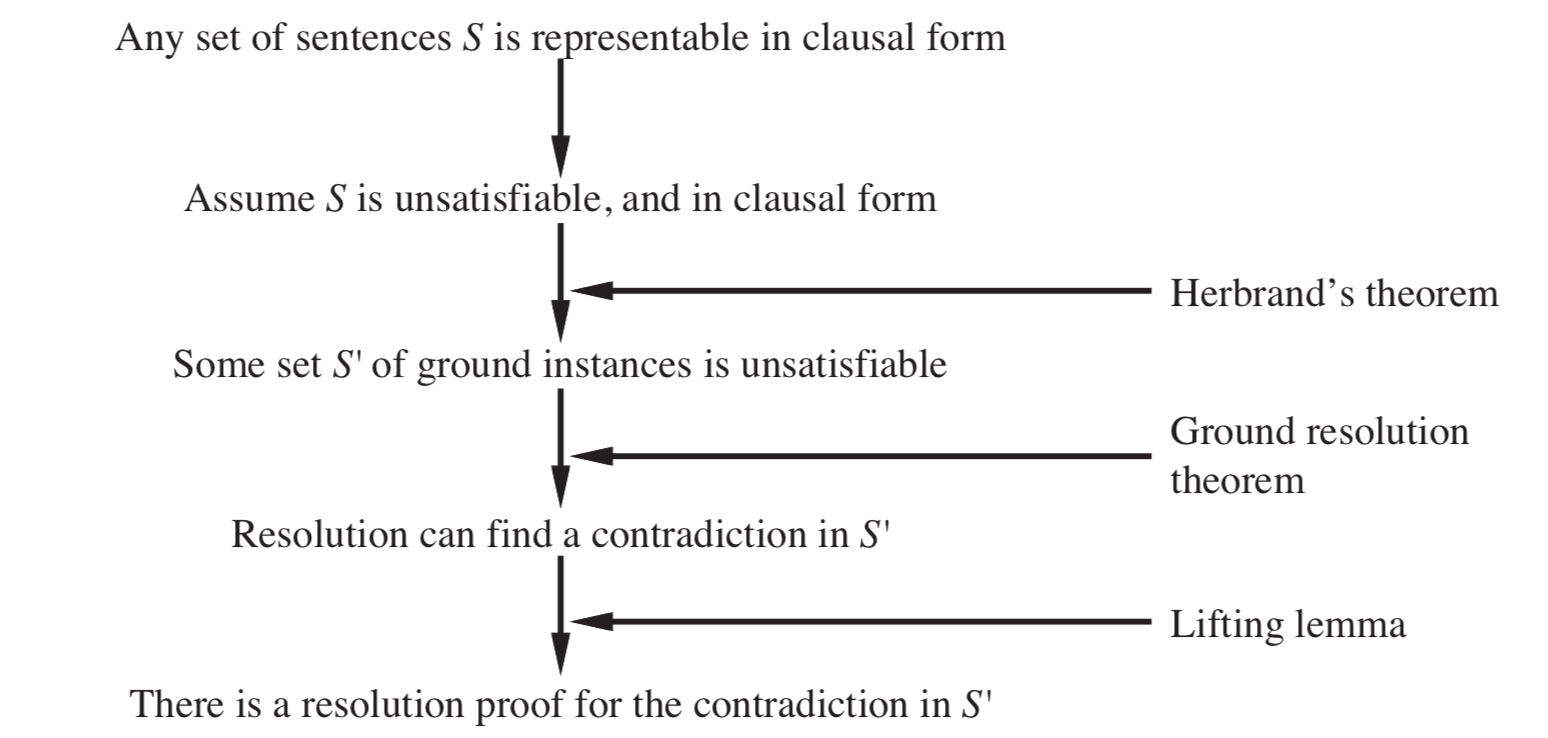
\includegraphics[scale=0.5]{images/fol_res_complete.png}
\caption{Structure of a completeness proof for resolution.}
\label{fig:fol_res_complete}
\end{figure}

Before explaining the proof we need to introduce some concepts.
\paragraph{Herbrand Universe}
Given a  set of clauses $S$ the Herbrand universe $H_S$ of those clauses is constructed in the following way:
\begin{itemize}
\item Following a function symbol if any.
\item Following a constant symbol if any.
\item 
\end{itemize}
Per example given $Parent(x,F(x,A))\vee Sibling(x,B)$ we can construct $Parent(Parent(A),F(F(A),A)),Parent(Parent(Parent(B)),F(B,F(B,A))),Sibling(A,Parent(B))....$.\\
That is we construct all the possible \textbf{ground terms} with the given function symbols ($Parent(x,y),Sibling(x,y)$), constant symbols ($A,B,F(A),Sibling(A,B)...$) and skolem formulas ($F(A,B),F(B,B),F(F(A),B)...$). 

\paragraph{Saturation} Given the set of ground terms $P$ obtained earlier, we generate the saturation of $S$ in respect to $P$, called $P(S)$, by applying all consistent substitution of ground term in $P$ with variables in $S$.

\paragraph{Herbrand Base}
\label{sec:herbrand_base}
The saturation of a set of clauses $S$ in respect to a Herbrand Universe is called a Herbrand Base, denoted $H_S(P)$ \footnote{Which is infinite.}.

\paragraph{Herbrand's Theorem}
The theorem says that:
\begin{center}
\textit{If a set S of clauses is unsatisfiable, then there exists a finite subset of $H_S(S)$ that
is also unsatisfiable.}
\end{center}
Let $S'$ be this finite subset of $H_S(S)$, we can use the ground resolution theorem (Section \ref{par:ground_res_theo}) to show that the resolution closure $RC(S')$ contains the empty clause. Hence we have demonstrated that there is \textit{always} a resolution proof involving some subset of $H_S(S)$, now we need to establish that there exists some proof involving $S$ itself \footnote{Note that the difference is that $S$ may not contain only ground clauses.}.

\paragraph{Lifting Lemma}
This lemma is used as a proof step from ground clauses up to general first-order clauses. The lemma says the following:
\begin{center}
Let $C_1$ and $C_2$ be two clauses with no shared variables, and let $C_1'$ and $C_2'$ be ground instances of $C_1$ and $C_2$. If $C'$ is a resolvent of $C_1$ and $C_2$ , then there exists a clause $C$ such that (1) $C$ is a resolvent of $C_1$ and $C_2$ and (2) $C'$ is a ground instance of $C$.
\end{center} 
For example, given the two clauses:
\[C_1=Heart(x,F(x,A))\vee Human(x)\]
\[C_2=\neg Heart(y,F(y,B))\vee Cyborg(y)\vee Oil(y,G(y,C))\]
We instantiate them with some ground terms (constant symbols only for simplicity):
\[C_1'=Heart(Goku,F(Goku,A))\vee Human(Goku)\]
\[C_2'=\neg Heart(C18,F(C18,B))\vee Cyborg(C18)\vee Oil(C18,G(C18,C))\]
Next we apply the resolution rule with $Human(x)$:
\[C'=Cyborg(C17)\vee Oil(C17,G(C17,C))\vee Human(C17)\]
And finally we generalize to get:
\[C'=Cyborg(y)\vee Oil(y,G(y,C))\vee Human(y)\]


\subsection{Resolution Strategies}
In the following we will analyze some strategies to make resolution more efficient.

\paragraph{Unit preference} Is the technique of preferring to use a single literal (unit clause) \footnote{For example $P$, not like $Q\vee R$.} to resolve against other clauses. This is because the length \footnote{Counted as the number of element in the disjunction.} of the resolution will be less than the other clause we used. For example, resolving:
\[\frac{P\vee \neg Q \vee R,\quad  F \vee \neg R \vee A}{P\vee \neg Q\vee F \vee A}\]
Which has length 4, higher than the two clauses used for resolution, while resolving:
\[\frac{P,\quad  F \vee \neg P \vee A}{ F \vee A}\]
That has length 2, shorter than the second clause.

\paragraph{Set of Support} We keep a set of clauses which are considered useful for the resolution inference, when we resolve something using an element from this set we add the resolvent to the set. Usually this set contains the negated query and generate a goal-directed proof tree.


\paragraph{Input Resolution} Is the technique of using a sentence from the input (either the query or the KB) and resolving it with another sentence. The \textbf{linear resolution} strategy is a slight generalization that allows $P$ and $Q$ to be resolved together either if $P$ is in the original KB or if $P$ is an ancestor of $Q$ in the proof tree. Linear resolution is complete.











\newpage


\section{Prolog}
Prolog is the major logic-based programming language \footnote{It is a sub-set of FOL.}, it uses a set of definite clauses written in a notation somewhat different from FOL.\\ 
For example:
\[American(x)\wedge \KinderEgg(y)\wedge Sells(x,y,z)\wedge Hostile(z)\Rightarrow Criminal(x)\]
becomes
\[criminal(X)\ :-\ american(X), kinderEgg(Y), sells(X,Y,Z), hostile(Z)\]
Note how the variables have \textit{uppercase} letters while the relationships are in \textit{lowercase}. As for the FOL case $criminal(X)$ is true if every atom in the premise $american(X), kinderEgg(Y), sells(X,Y,Z), hostile(Z)$ is also true.\\

\paragraph{An Example}
We write a program with the following rules:
\begin{enumerate}
\item $append([\ ],Y,Y)$: if I append to an empty list $[\ ]$ another list $Y$, then the result will be the same list $Y$.
\item $append([A|X],Y,[A|Z]) :- append(X,Y,Z)$: the premises (on the right) says that appending $X$ to $Y$ produces $Z$, if this is true then appending $Y$ to $[A|X]$ \footnote{This notation denotes a list whose first element is $A$ and rest is $X$.} will output $[A|Z]$. 
\end{enumerate}
And we query $append(X,Y,[1,2])$ (what can be the values of $X,Y$ so that, if I append them, I have $[1,2]$?) and obtain:
\begin{itemize}
\item $X=[\ ]\quad Y=[1,2]$
\item $X=[1]\quad Y=[2]$
\item $X=[1,2]\quad Y=[\ ]$
\end{itemize}


\subsection{Efficient Implementation}
There are two modes of operation for the Prolog program. 


\begin{figure}[H]
\centering
\fbox{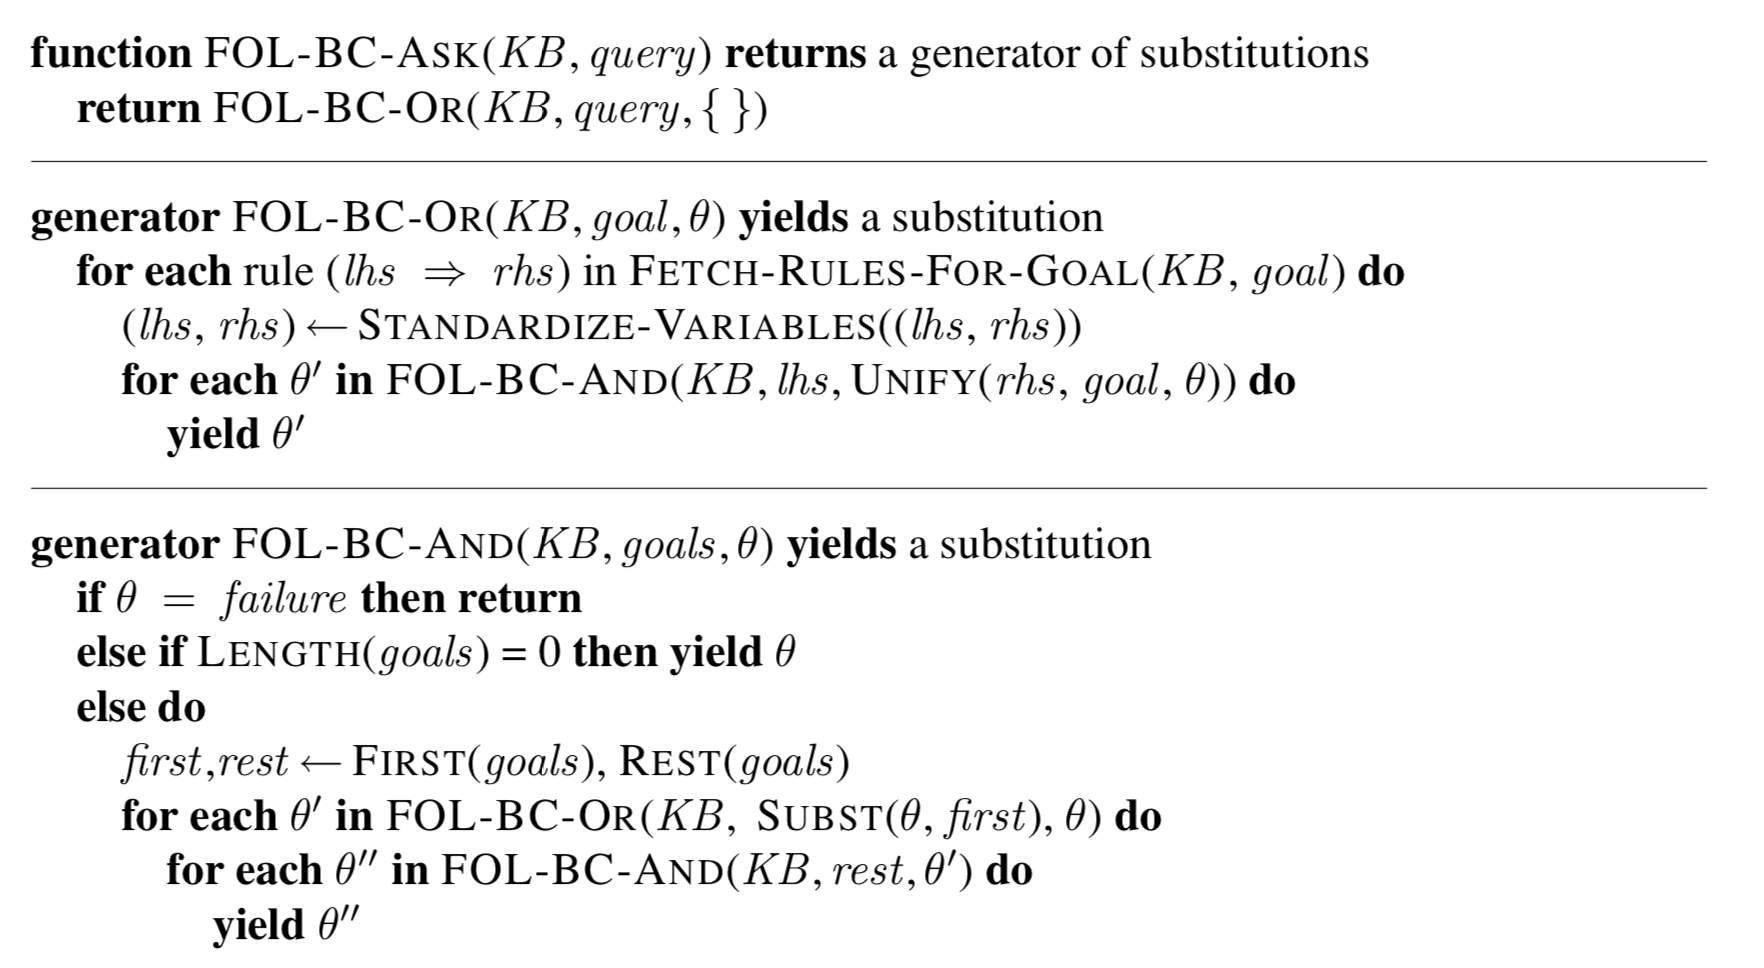
\includegraphics[scale=0.5]{images/prolog_interpreted.png}}
\caption{Abstract Interpreted Prolog Mode}
\label{fig:interpreted_prolog}
\end{figure}

\paragraph{Interpreted}
The algorithm works as shown in Figure \ref{fig:interpreted_prolog} with two major improvements:
\begin{itemize}
\item The presence of a \textbf{global stack}\footnote{Remember that a stack is the implementation of a depth-first search.} of choice points to keep track of multiple possibilities to consider .
\item The use of a \textbf{trail} in which logic variables \footnote{Variables that remember their current bindings .} are kept. So when a branch fails the algorithm removes the last bounded variable and continues with the trail \textit{without} re-instantiating a substitution for each variable.
\end{itemize}


\paragraph{Compiled} In this mode the Prolog program becomes  an inference procedure for a specific set of clauses, so it knows what clauses match the goal. Prolog basically generates a miniature theorem prover for each different predicate, thereby eliminating much of the overhead of interpretation. ??????????????????

\paragraph{Parallelization} There are two principal sources of parallelism. The first, called \textbf{OR} parallelism, comes from the possibility of a goal unifying with many different clauses in the knowledge base. Each gives rise to an independent branch in the search space that can lead to a potential solution, and all such branches can be solved in parallel. The second, called textbf{AND} parallelism, comes from the possibility of solving each conjunct in the body of an implication in parallel.

\subsection{Redundant inference and infinite loops}
Since Prolog works with backward chaining, hence using a depth-first search, some issues may arise. Specifically the problem of infinite paths makes Prolog \textbf{incomplete} as a theorem prover for definite clauses because it fails to prove sentences that are entailed. 

\paragraph{An example}
Given two implementation of the same problem:
\begin{enumerate}
\item The first one:
	\begin{itemize}
	\item path(X,Z) :- link(X,Z)
	\item path(X,Z) :- path(X,Y), link(Y,Z)
	\end{itemize}
\item The second one:
	\begin{itemize}
	\item path(X,Z) :- path(X,Y), link(Y,Z)
	\item path(X,Z) :- link(X,Z)
	\end{itemize}
\end{enumerate}

Since Prolog chooses the clauses in the order of implementation, the resulting search tree for the second implementation will be an infinite loop, as shown in Figure \ref{fig:prolog_tree}.


\begin{figure}[H]
\centering
\fbox{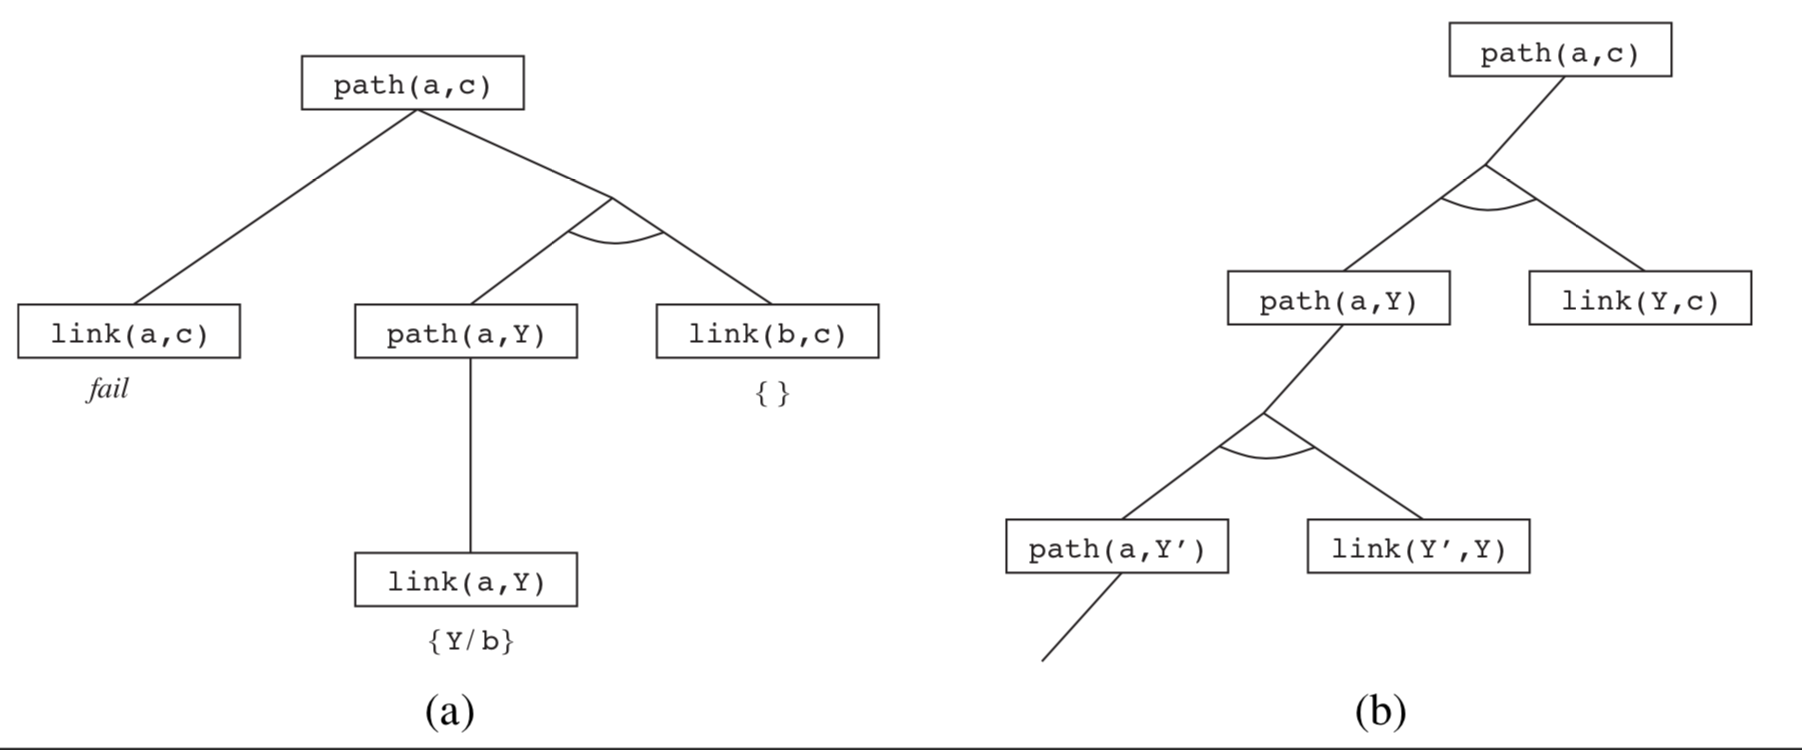
\includegraphics[scale=0.5]{images/prolog_tree.png}}
\caption{Abstract Interpreted Prolog Mode}
\label{fig:prolog_tree}
\end{figure}

\newpage

\section{Non Monotonic Reasoning}

In classical logic the more facts we have, the more conclusions we can draw, this property is known as \textbf{Monotonicity}, which can be formalized as:
\[if\ \Delta \subset \Gamma:\ Cn(\Delta)\subset Cn(\Gamma)\]
In which $Cn(x)$ is a classical conclusion based on some st of premises $x$. So if we have a set of facts $\Delta$ which is a subset of $\Gamma$, then the new facts in gamma will have no effects on the conclusions in $Cn(\Delta)$; that is $  Cn(\Delta)\subset Cn(\Gamma)$.\\
On the other hand \textbf{non-monotonicity} models a common behavior in humans minds: the changing of one's idea \footnote{Where more information leads us to retract previous conclusions.}. A classical example would be:\\ 
\textit{Suppose I tell you ‘Tweety is a bird’}.\\
\textit{You might conclude ‘Tweety flies’}.\\
\textit{I then tell you ‘Tweety is an emu’}.\\
\textit{You conclude ‘Tweety does not fly’}.\\

Moreover there are some other problem with classical logic such as:
\begin{itemize}
\item It is usually not possible to write down all we would like to say about a domain.
\item  Inferences in classical logic simply make implicit knowledge explicit; we would also like to reason with tentative statements.
\item Sometimes we would like to represent knowledge about something that is not entirely true or false; uncertain knowledge.
\end{itemize}

\subsection{Closed World Reasoning}
The close world assumption, CWA for short says the following:\\
\textit{There are many more false things than true things. If something is true and relevant, it has been put into the KB. So, if something is not present in the KB, it can reasonably be assumed to be false.}\\
The CWA completes a non-closed KB \footnote{On the contrary a complete KB is one in which for every ground atom in the language, either the atom or its negation appears in the KB. } by including the negation of a ground atom whenever the atom does not follow from the KB.\\
In other words, if we have no evidence as to the truth of a ground atom, we assume that it is false. This can be formalized as:
\[CWA(KB)=KB^+=KB \cup \Delta_{asm}\]
Where $\Delta_{asm}$ is the assumption set containing all the negative literals $L$ if $L$ is not derivable from the KB:
\[\Delta_{asm}=\{\neg L | L\ if\ L\ is\ positive\ literal\ and\ KB \nvDash L\}\]
Another way of characterizing the assumption set is using the Herbrand Base \textit{HB(KB)} (Section \ref{sec:herbrand_base}):
\[\Delta_{asm}=\{\neg L : KB \nvDash L\ and\ L\in HB(KB)\}\]

\paragraph{An Example}
Let the KB be made of two formulas:
\begin{itemize}
\item $\forall x\ P(x) \Rightarrow Q(x)$
\item $P(a)\wedge R(b)$
\end{itemize}
We have that the Herbrand Base of the KB is:
\[HB(KB)=\lbrace P(a), Q(a), R(a), P(b), Q(b), R(b) \rbrace\]
So our set of assumption would be:
\[\Delta_{asm}=\lbrace \neg R(a), \neg P(b), \neg Q(b) \rbrace\]


\paragraph{Completeness of CWA}
We can show that CWA produces a complete KB since we have that:
\[\forall \alpha, KB^+ \modules \alpha\ or\ KB^+ \modules \neg \alpha\]
Where $\alpha$ can be either an atom or formula. 

\paragraph{Consistency of CWA}
Let KB be a consistent \footnote{Consistent means that I cannot have both $P(a)$ and $\neg P(a)$ in the KB at the same time.} set of formulas. $CWA(KB)$ is consistent iff any clause $C$ that
is formed of positive ground literals $P_i$ that can be deduced from the KB, such as $C=P_1\vee...\vee P_2$; every $C$ contains at least one positive ground literal $P_i$ that can be deduced from the KB.


\paragraph{Generalized CWA}
Let a KB be the following:
\begin{itemize}
\item $Course(AI) \wedge Course(MachineLearning)$
\item $Student(Nardi) \vee Professor(Nardi)$
\end{itemize}
If we apply CWA to the KB we have an inconsistency. However it is still reasonable (and consistency preserving) to assume that \textit{AI} and \textit{MachineLearning} are neither students nor professors, 
and that and that \textit{Nardi} is not a course is not a course. So we can use Generalized CWA [GCWA] in the following way:
\[GCWA(KB)=KB\cup \Delta_{asm}\]
Where $\Delta_{asm}= \lbrace \neg L | L$ \textit{is a positive literal and there is no positive clause C
such that} $KB \models L\wedge C and KB \nVDash C \rbrace$.\\
So an atom $L$ can be assumed to be false only if it is the case that whenever a disjunction of atoms, including that atom, is entailed by KB; the smaller disjunction without the atom is also entailed.\\
For the previous example we have that, $GCWA(KB)$:
\begin{itemize}
\item $\neg Course(Nardi)$
\item $\neg Student(AI), \neg Student(MachineLearning)$
\item $\neg Professor(AI), \neg Professor(MachineLearning)$
\end{itemize}

\subsection{Negation}
Given a KB and an atom $A$, the \textbf{negation as failure} says the following:\\
\textit{If from the KB we do not prove $A$, then from the KB we deduce $\neg A$.}\\


\subsubsection{Semantic of stable models}
The basic idea is to design a model of a certain KB as a \textbf{canonical} model, i.e. this models determine which answer to a given query is considered correct. For example having KB:
\begin{itemize}
\item $P(1),Q(2)$
\item $P(x) \Rightarrow Q(x)$
\end{itemize}
Have two models:
\begin{enumerate}
\item $M_1=\lbrace P(1), Q(1), Q(2) \rbrace$
\item $M_2=\lbrace P(1), Q(1), Q(2), P(2)\rbrace$ \footnote{This one is exactly equal to the Herbrand Base of KB.}
\end{enumerate}
We can see how 1) is a minimal model which is also unique in KB which are in Horn Normal Form (Section \ref{subsubsec:horn}). But when we introduce negations then we loose the HNF, thus there is no unique minimal model.\\

\paragraph{Grounding} is the technique of replacing a clause with its ground instance.

\paragraph{Negation Elimination} Given a set $M$ of atoms of KB, the reduct $KB_M$ is obtained by eliminating:
\begin{itemize}
\item all the clauses that in the body have a negated atom of M;
\item all the negative literals not in M.
\end{itemize}
Now we have that $KB_M$ is negation-free thus having an unique minimal model. If this model coincide with $M$ then we can say that $M$ is a \textbf{stable set} of the KB.\\

\paragraph{Theorem}
\textit{Every stable set of a KB is a minimal Herbrand model of KB}.\\
The intuitive meaning is as follows:\\
IF $M$ is a set of ground atoms that an Agent $A$ considers to be true, then any rule that has a sub-goal $\neg B$ with $B \in M$ is, form the agent point of view, useless; furthermore, any sub-goal $\neg B$ with $B \notin M$ is, from the agent point of view, trivial. Then $A$ can simplify the premises in the KB and replace them with $KB_M$. If $M$ happens to be precisely the set of atoms that logically follows from $KB_M$ then $A$ is being rational.\\

The stable model semantic is defined for logic program if they have exactly one stable model, and it declares that model to be a canonical model.




\newpage
\changelocaltocdepth{2}

\section{Exercises}

\subsection{First Order Logic}

\subsubsection{Ex1}
Choose a suitable vocabulary of constant and predicate symbols then represent the following sentences in FOL:
\begin{enumerate}
\item Steve likes easy classes
\item Violin classes are not easy
\item Every class of Percussion is easy
\item The class of “Afro Drums” is a class of Percussion
\item The class of “Violin for pre-school Kids” is a class of Violin
\end{enumerate}
The KB will look something like this:
\begin{enumerate}

\item $\forall x\ Class(x)\wedge Easy(x) \Rightarrow Likes(Steve,x)$
\item $\forall x\ Class(x)\wedge Violin(x) \Rightarrow \neg Easy(x)$
\item $\forall x\ Class(x)\wedge Percussion(x) \Rightarrow Easy(x)$
\item $Class(AfroDrums), Percussion(AfroDrums)$
\item $Class(ViolinKids), Violin(ViolinKids)$

\end{enumerate}
Notice that the second formula is not a definite clause but a goal clause (Section \ref{subsubsec:horn}). This makes the KB in Horn normal Form.


Can we infer that Steve likes the class of Afro Drums ($Likes(Steve,x),\ \{x/AfroDrums\}$)?
\begin{itemize}
\item using Modus Ponens
\item using Resolution
\end{itemize} 


\paragraph{Using Modus Ponens}
The steps are the following:
\begin{itemize}
\item Use MP for 3,4:
\[\frac{Class(AfroDrums), Percussion(AfroDrums),\quad [Class(x)\wedge Percussion(x) \Rightarrow Easy(x)]}{Easy(AfroDrums)}\]
With the substitution $\theta=\lbrace x/AfroDrums \rbrace$. Then add  $Easy(AfroDrums)$ to the KB.

\item Finally use MD on 1 using the ground term we just deducted from the previous step:
\[\frac{Easy(AfroDrums),Class(AfroDrums),\quad [\forall x\ Class(x)\wedge Easy(x) \Rightarrow Likes(Steve,x)]}{Likes(Steve,AfroDrums)}\]
\end{itemize}


\paragraph{Resolution}
We first need to bring the KB in  Skolem Normla Form SNF (Section \ref{sec:skolemNF}) \footnote{Note that there are no existential quantifiers, so there is no need for skolem unctions. On the other hand SNF is not only about skolem functions, universal quantifiers are treated too with $UI$ (Section \ref{subsubsec:UI}). }.

\begin{enumerate}
\item $\neg Class(x) \vee \neg Easy(x) \vee Likes(Steve,x)$
\item $\neg Class(y) \vee \neg Violin(y) \vee Easy(y)$
\item $\neg Class(z) \vee \neg Percussion(z) \vee Easy(z)$
\item $\neg q=\neg Likes(Steve,g)$
\end{enumerate}

So we end up with three clauses and can start the resolution mechanism. We want to derive the query $q=Likes(Steve,AfroDrums)$ from the KB, $KB\vdash_{\mathcal{R}}q$, hence we need to prove that $(KB \vee \neg q) \vdash_{\mathcal{R}} \{\}$.\\
First we use the 1,4, with the substitution $\theta=\lbrace x/AfroDrums\rbrace$ and get:
\[\frac{\lbrace \neg Class(x), \neg Easy(x), Likes(Steve,x)\rbrace\quad \lbrace \neg Likes(Steve,g)\rbrace}{\lbrace \neg Class(AfroDrums), \neg Easy(AfroDrums) \rbrace}\]
Note that this is a case of \textbf{binary resolution} (Section \ref{sec:binaryresolution}). Next we use the facts in the KB.
\[\frac{\lbrace \neg Class(AfroDrums),\neg Easy(AfroDrums) \rbrace,\quad \lbrace Class(AfroDrums) \rbrace}{\lbrace \neg Easy(AfroDrums) \rbrace}\]
And finally we use:
\[\frac{\lbrace \neg Easy(AfroDrums) \rbrace,\quad \lbrace Easy(AfroDrums) \rbrace}{\lbrace \rbrace}\]
Which entails the empty clause, thus $(KB \vee \neg q) \vdash_{\mathcal{R}} \{\}$ is true, thus $KB\vdash_{\mathcal{R}}q$.

\subsubsection{Ex2}
Let $Gov$ , $Univ$, $Luca$, $Bill$ be constant symbols, and let

\begin{itemize}
\item $Prof(x)$
\item $Student(x)$
\item $Unhappy(x)$
\item $CutFund(x,y)$
\item $FailExam(x,y)$
\end{itemize}
be unary and binary predicate symbols.

Given:
\begin{itemize}
\item If the Government cuts the funds to Universities, professors are unhappy.
\item If professors are unhappy all students fail their exams.
\item The Government cuts the funds to Universities.
\item $Luca$ is a professor and $Bill$ is a student
\end{itemize}

The exercise demand to:
\begin{enumerate}
\item Express in FOL the above KB.
\item Prove that Bill fails Luca’s exam using both Modus Ponens and Resolution
\end{enumerate}

\paragraph{KB in FOL}
\begin{enumerate}
\item $Prof(Luca),Student(Bill)$
\item $\forall x\ \forall y\ [Prof(x) \wedge Unhappy(x)\wedge Student(y)]\Rightarrow [FailExam(x,y)]$
\item $\forall x\ CutFund(Gov,Univ) \wedge Prof(x) \Rightarrow Unhappy(x)$
\item $CutFund(Gov,Univ)$
\end{enumerate}

\paragraph{Modus Ponens}
Given the facts in 1) and 4) we can use MP on formula number 3:
\[\frac{[CutFund(Gov,Univ),Prof(Luca)],\quad [\forall x\ CutFund(Gov,Univ) \wedge Prof(x) \Rightarrow Unhappy(x)]}{Unhappy(Luca)}\]
with the substitution $\theta=\lbrace x/Luca \rbrace$ and add the consequence $Unhappy(Luca)$ to the KB.\\
Finally we can use MD on the facts we have and on formula number 2):
\[\frac{[Prof(Luca),Unhappy(Luca),Student(Bill)],\quad [\forall x\ \forall y\ [Prof(x) \wedge Unhappy(x)\wedge Student(y)]\Rightarrow [FailExam(x,y)]]}{Fail(Luca, Bill)}\]
Proving that Bill will fail Luca's exam.

\paragraph{Resolution}
First we need to transform our KB into CNF (Section \ref{subsec:cnf}).\\
For formula 2 we have:
\begin{itemize}
\item $\forall x\ \forall y\ [Prof(x) \wedge Unhappy(x)\wedge Student(y)]\Rightarrow [FailExam(x,y)]$
\item Remove universal quantifiers with UI (Section \ref{subsubsec:UI}):
\[[Prof(x) \wedge Unhappy(x)\wedge Student(y)]\Rightarrow FailExam(x,y)\]
\item Remove implication:
\[\neg [Prof(x) \wedge Unhappy(x)\wedge Student(y)]\vee FailExam(x,y)\]
\item Move negation inwards:
\[\neg Prof(x) \vee \neg Unhappy(x)\vee \neg Student(y)\vee FailExam(x,y)\]
\item Write in clause form:
\[C_1=\lbrace \neg Prof(x), \neg Unhappy(x), \neg Student(y), FailExam(x,y)\rbrace\]
\end{itemize}
For 3) do something similar and get:
\[C_2= \lbrace \neg CutFund(Gov,Univ),\neg Prof(z), Unhappy(z) \rbrace\]
Note that I've changed the variables from $x$ to $z$ to avoid confusion for later substitution.\\
Finally get:
\[C_3,C_4,C_5=\lbrace Prof(Luca) \rbrace,\ \lbrace Student(Bill) \rbrace,\ \lbrace CutFund(Gov,Univ) \rbrace,\]

Now we query to the KB $q= FailExam(Luca,Bill)$, thus adding the negated query to the KB.\\
First we resolve $C_3,C_5$ with $C_2$, using the substitution $\theta=\lbrace z/Luca \rbrace$:
\[\frac{[C_3,C_5],\quad C_2}{C_6=\lbrace Unhappy(Luca) \rbrace}\]
Then we resolve $C_6,C_3,C_4$ with $C_1$, using the substitution $\theta= \lbrace x/Luca, y/Bill \rbrace$ and get:
\[\frac{[C_3,C_4,C_6],\quad C_1}{\lbrace \rbrace}\]
The empty clause, which prove that $(KB \wedge \neg q)\vdash \{\}$, thus $KB \vdash_{\mathcal{R}} q$.


\subsubsection{Ex3}
Tell whether or not the following pairs of expressions unify. Describe the unification process step by step:
\begin{enumerate}
\item $f(g(a, X), g(X, b)) = f(g(a, b, c, d))$
\item $f(g(a, X), g(Y, Y )) = f(g(a, b), g(f(a), f(Z)))$
\item $f (cons(cons(a, b))) = f (cons(cons(a, nil))$
\end{enumerate}

Number one is \textbf{not unifiable} since the predicate $f()$ has arity 2 (2 arguments) in the first part of the unification, while it has only one in the second.\\

Number two is \textbf{unifiable}. First the arity of both the predicates $f,g$ are the same in the two parts of the equation. The first thing we have to unify is :
\[g(a,X)=g(a,b)\]
Which yields $\theta=\lbrace X/b \rbrace$. Then we nned to look at :
\[g(Y,Y)=g(f(a),f(Z))\]
If we notice that $Z$ is a variable which can assume any value and that we must have the two arguments of $g$ the same for $g(Y,Y)$ we just use $Z=a$ and get:
\[g(Y,Y)=g(f(a),f(a))\]
And then we substitute with $Y=f(a)$.\\

Number three is written in a weird way, but if we look at Nardi's slides we can interpret it to be (maybe):
\[ f([[a|b]|[]])=f([[a|[]]|[]]) \]
Which is \textbf{not unifiable} since Prolog says so (seriously I couldn't understand it).


\subsubsection{Ex4}
Answer the following questions:
\begin{enumerate}
\item  Is $P(c)$ the Skolemized version of $\exists x\ P(x)$?
\item  Is $\forall x\ P(c,x)$ the Skolemized version of $\forall x\ \exists y\ P(y,x)$?
\item  Is $\forall x\ P(f(x),x)$ the Skolemized version of $\forall x\ \exists y\ P(y,x)$?
\item  Is $P(c_1,c_2)$ the Skolemized version of $\exists x\ \exists y\ P(x,y)$?
\item  Is $\forall y\ P(c_1,y,f(y))$ the Skolemized version of $\exists x\ \forall y\ \exists z\ P(x,y,z)$?
\item  Is $P(x,y,f(y))$ the Skolemized version of $\forall x\ \forall y\ \exists z\ P(x,y,z)$?
\end{enumerate}

Answers:
\begin{enumerate}
\item No, that would be the EI (Section \ref{subsubsec:EI}) of the original formula \footnote{Given that $c$ does not appear in the KB.}. A Skolemized version would be $P(f(x))$, where $f$ does not appear in the KB.
\item No, that would be the EI of the original formula. A Skolemized version would be $P(f(x),x)$.
\item Yes.
\item Yes, since the existential quantifiers [EQ] do not depend on any universal quantifier [UQ], so we can use EI to remove them.
\item Yes, because the first EQ does not depend on any UQ, hence we can use the EI. The second  EQ depends on the UQ controlling $x$ so we need a function which depends on $x$.
\item No, because $z$ depend both on $y$ and $x$ so the correct skolem function would take into account both the UQ. A Skolemized version would be $P(x,y,f(x,y))$
\end{enumerate}

\subsubsection{Ex 5}
Given:
\begin{itemize}
\item The textbooks of class CA are easy
\item The textbooks of class CB are difficult
\item  Mary studies (all and only) easy books
\item  Mary passes the exam of a class if she studies at least a textbook for that class
\item  Russel&Norvig is a textbook for class CA
\item  Tenenbaum is a textbook for class CB
\end{itemize}

Do the following:
\begin{enumerate}
\item Translate the sentences in FOL, in CNF and tell if it is Horn 
\item  Prove, using Resolution, that Mary passes an exam, by adding the appropriate knowledge (if needed)
\end{enumerate}


\paragraph{Part 1}
The first order logic KB would be:
\begin{itemize}
\item $\forall x\ Ca(x)  \Rightarrow Easy(x)$
\item $\forall x\ Cb(x) \Rightarrow \neg Easy(x)$
\item $\forall x\  Easy(x) \Rightarrow Study(Mary,x)$
\item $\exists x\ Study(Mary,x) \wedge Passes(Mary,x)$
\item $Ca(R&N), CB(Tb)$
\end{itemize}

The CNF would be:
\begin{itemize}
\item $C_1= \lbrace \neg Ca(x), Easy(x) \rbrace$
\item $C_2= \lbrace \neg Cb(x), \neg Easy(x) \rbrace$
\item $C_3= \lbrace \neg Easy(x), Study(Mary,x) \rbrace$
\item $C_4= \lbrace Study(Mary,B) \rbrace$, where we used EI (Section \ref{subsubsec:EI}) to refer to a generic book $B$ that Mary studies.
\item $C_5= \lbrace Passes(Mary,B) \rbrace$, in this case we are not making any difference between the exam that Mary passes and the book she uses to study. We will refer to the exam based on R&N or on Tb.
\item $C_6= \lbrace Ca(R&N) \rbrace$
\item $C_7= \lbrace Cb(Tb) \rbrace$
\end{itemize}
We can tell that the KB is in Horn form since all the clauses have \textbf{at most one} positive literal (Section \ref{subsubsec:horn}).

\paragraph{Part 2}
First we need to add some knowledge to the KB in order to make Mary study something. We add the sentence:\\
\textit{Mary studies R&N.}\\
Which, in FOL, is equivalent to say : $Study(Mary,R&N)$.\\
Which, in CNF, is :$C_8=\lbrace Study(Mary,R&N) \rbrace$.\\
In order to prove that Mery passes the R&N exam we need to query $q=Passes(Mary,R&N)$ to the KB, thus we need to prove that $(KB \wedge \neg q) \vdash \{\}$. The resolution follows these steps:
\begin{enumerate}
\item Resolve $\neg q$ with $C_3$, using the substitution $\theta=\lbrace x/R&N \rbrace$:
\[\frac{\neg Passes(Mary,R&N),\quad \lbrace \neg Easy(x), Study(Mary,x) \rbrace}{C_9=\lbrace \neg Easy(R&N) \rbrace}\]
\item Resolve $C_9$ with $C_1$,  using the substitution $\theta=\lbrace x/R&N \rbrace$:
\[\frac{\neg Easy(R&N),\quad \lbrace \neg Ca(x), Easy(x) \rbrace}{C_{10}=\lbrace \neg Ca(R&N) \rbrace}\]

\item Finally resolve $C_{10}$ with the fact $C_6$ and obtain the empty clause.
\end{enumerate}

\vfill

\subsection{MidTerms}
\subsubsection{M1}


$D$ is the gardener of a vegetable garden $V$ and a flower garden $F$. Gardens that have a gardener are beautiful iff their gardener waters them. Every gardener waters his gardens, if water is available, which is fortunately the case for $D$.
\begin{enumerate}
\item  Define a vocabulary (i.e., constant, function and predicate symbols) and represent the following sentences in first order logic.
\item Translate the sentences in clausal form.
\item show using resolution that V and F are beautiful.
\end{enumerate}


\paragraph{Part 1}
Our vocabulary will have the following predicates:
\begin{itemize}
\item $Garden(x)$ express that $x$ is a garden.
\item $Gardener(x,y)$ express that $x$ is the gardener of garden $y$.
\item $HasWater(x)$ express that the gardener $x$ has water.
\item $Watered(x)$ express that the garden $x$ has been watered.
\item $Beautiful(x)$ express that the garden $x$ is beautiful.
\end{itemize}

Given this predicates we can express the sentence in FOL:
\begin{enumerate}
\item First we express the ground terms:
\[ Garden(V), Garden(F), Gardener(D,V), Gardener(D,F), HasWater(D)\]
\item Then we need to express that if a gardener $g$ of some garden $x$ \footnote{We know that a gardener can have multiple gardens, so we use $\forall$ gardens.} has water, then the $x$ will be watered:
\[\forall g \forall x[\ HasWater(g)\wedge Gardener(g,x)\Rightarrow Watered(x)]\]
\item Next we formulate that for every garden $x$, if $x$ has a gardener $y$ \footnote{We can use the existential quantifier since we're interested in knowing if there exist some gardener for $x$. } and $x$ is watered, then $x$ is beautiful.
\[\forall x\ [Garden(x)\wedge [\exists y\ Gardener(y,x)]\wedge Watered(x)\Rightarrow Beautiful(x)]\]
\end{enumerate}

\paragraph{Part 2}

From 2, we have:
\begin{itemize}
\item Use $UI$ (Section \ref{subsubsec:UI}) to remove universal quantifiers:
\[ HasWater(g)\wedge Gardener(g,x)\Rightarrow Watered(x)\]
\item Remove implication:
\[\neg HasWater(g)\vee \neg Gardener(g,x)\vee Watered(x)\]
\item Use clausal form:
\[\lbrace \neg HasWater(g), \neg Gardener(g,x), Watered(x)\rbrace\]
\end{itemize}

From 3, we have:
\begin{itemize}
\item Remove existential quantifier using a skolem function (Section \ref{sec:skolemNF}) $G(x)$:
\[\forall x\ [Garden(x)\wedge  Gardener(G(x),x) \wedge Watered(x)\Rightarrow Beautiful(x)]\]
\item Remove universal quantifier using $UI$:
\[Garden(x)\wedge  Gardener(G(x),x) \wedge Watered(x)\Rightarrow Beautiful(x)\]
\item Remove implication:
\[\neg Garden(x)\vee \neg Gardener(G(x),x) \vee \neg Watered(x)\vee Beautiful(x)\]
\item Use clausal form:
\[\lbrace \neg Garden(x), \neg Gardener(G(x),x) , \neg Watered(x), Beautiful(x)\rbrace\]
\end{itemize}

Our KB now looks like this:
\begin{itemize}
\item $C_1=\lbrace \neg HasWater(g), \neg Gardener(g,x), Watered(x)\rbrace$
\item $C_2=\lbrace \neg Garden(x), \neg Gardener(G(x),x) , \neg Watered(x), Beautiful(x)\rbrace$
\item $C_3,C_4,C_5,C_6,C_7=Garden(V), Garden(F), Gardener(D,V), Gardener(D,F), HasWater(D)$
\end{itemize}



\paragraph{Part 3}
We want to query $q_1=Beautiful(V)$ and $q_2=Beautiful(F)$. Let us start with $q_1$, so we want to show that $(KB \wedge \neg q_1)\vdash_{\mathcal{R}} \{\}$:
\begin{itemize}
\item We first use resolve $C_7$ with $C_1$, with the substitution $\theta=\{g/D\}$
\[\frac{ HasWater(D),\quad \lbrace \neg HasWater(g), \neg Gardener(g,x), Watered(x)\rbrace}{C_8=\lbrace \neg Gardener(D,x), Watered(x)\rbrace}\]
Adding it to the KB.
\item Since we're interested in $V$ we resolve $C_5$  with $C_8$, with the substitution $\theta=\{x/V\}$:
\[\frac{Gardener(D,V),\quad \lbrace \neg Gardener(D,x), Watered(x)\rbrace}{C_9=\lbrace \neg Watered(V)\rbrace}\]
\item Until now we have used only \textbf{binary resolution}, now we will use the general one. Given $C_3,C_5,C_9,\neg q_1$ we can resolve them with $C_2$ with the substitution $\theta=\{x/V\}$ we resolve with $\{\}$ thus proving that $(KB \wedge \neg q_1)\vdash_{\mathcal{R}} \{\}$.
\end{itemize}
Same thing goes for $q_2$.


\subsubsection{M2}
Tell which one among the following First Order Logic formulas is an adequate representation of the sentence (and provide an explanation of the answer):
Italians are happy if the Italian National team wins the world cup.
\begin{enumerate}
\item $\forall x\forall y\ [Italian(x)\Rightarrow [WinWc(y)\Rightarrow Happy(x)]]$
\item $\forall x\forall y\ [Italian(x)\wedge WinWc(y)]\Rightarrow Happy(x)]$
\item $\forall x\exists y\ [Italian(x)\wedge WinWc(y)]\Rightarrow Happy(x)]$
\item $\forall x\ [[Italian(x)\wedge WinWc(National)]\Rightarrow Happy(x)]$
\item $\forall x\ [[Italian(x)\wedge WinWc(National)]\wedge Happy(x)]$
\item $\forall x\ [[Italian(x)\wedge Happy(x)]\Rightarrow  WinWc(National)]$
\end{enumerate}

We can rule out the first two (1,2) since there is only one Italian National, so no need for an universal quantifier for ($WinWc(y)$).\\
Number 5 is no good since universal quantifier works with implication rather than $conjunction$ (Section \ref{sec:quantifiers}).\\
Number 6 has no sense, since it saying: if Italians are happy then the national will win.\\
Number 4 is good since the sense is correct.\\
Finally number 3 is wrong. On the other hand it would be good  if the existential quantifier was to be moved outside the scope of the universal one; in this case we could have used $EI$ (Section \ref{subsubsec:EI}) to get:
$\forall x\ [Italian(x)\wedge WinWc(N)]\Rightarrow Happy(x)]$
And we could get exactly number 4 with the substitution $\theta=\{N/National\}$.

\subsubsection{M3}
$D$ is the advisor of two PhD students $F$ and $A$, who are both motivated. PhD students who have an advisor are successful iff their advisor cares about them. Every advisor cares about his/her students, when they are motivated.
\begin{enumerate}
\item Define a vocabulary (i.e., constant, function and predicate symbols) and represent the following sentences in first order logic.
\item Translate the sentences in clausal form.
\item Show using resolution that F and A are successful
\end{enumerate}


\paragraph{Part 1}

Our vocabulary will have the following predicates:
\begin{itemize}
\item $Student(x)$ express that $x$ is a student.
\item $Advisor(x,y)$ express that $x$ is the advisor of student $y$.
\item $Motivated(x)$ express that the person $x$ is motivated.
\item $Cares(x,y)$ express that the  $x$ cares about $y$.
\item $Successful(x)$ express that the person $x$ is successful.
\end{itemize}


Given the sentence we can translate it into FOL:
\begin{enumerate}
\item Some ground terms:
\[Student(F),Student(A),Advisor(D,F),Advisor(D,A), Motivated(F),Motivated(A)\]
\item For every student $x$, there is one or more advisors $y$, if the advisor cares about the student then $x$ will be successful.
\[\forall x\exists y\ [Cares(y,x)\wedge Advisor(y,x)]\leftrightarrow Successful(x)\]
\item Finally for every student $y$ and for every advisor $x$, if $y$ is motivated and $x$ is the advisor of $y$, then $x$ cares about $y$.
\[\forall x \forall y [Advisor(x,y)\wedge Motivated(y)]\Rightarrow Cares(x,y)\]
\end{enumerate}

\paragraph{Part 2}

From 2 we have:
\begin{itemize}
\item Use skolem function $Adv(x)$ to remove the existential quantifier:
\[\forall x\ [Cares(Adv(x),x)\wedge Advisor(Adv(x),x)]\leftrightarrow Successful(x)\]

\item Use $UI$ (Section \ref{subsubsec:UI}) to remove universal quantifiers:
\[ [Cares(Adv(x),x)\wedge Advisor(Adv(x),x)]\leftrightarrow Successful(x)\]
\item Remove double implication:
\[ [Cares(Adv(x),x)\wedge Advisor(Adv(x),x)]\Rightarrow Successful(x)\]
And 
\[ Successful(x)\Rightarrow [Cares(Adv(x),x)\wedge Advisor(Adv(x),x)] \]
\item Remove implication :
\[ \neg Cares(Adv(x),x)\vee \neg Advisor(Adv(x),x)\vee Successful(x)\]
And
\[ \neg Successful(x)\vee [Cares(Adv(x),x)\wedge Advisor(Adv(x),x)] \]
\item Use "OR" distribution on second term:
\[ [\neg Successful(x)\vee Cares(Adv(x),x)]\wedge [\neg Successful(x)\vee Advisor(Adv(x),x)] \]
\item Use clausal form:
\[\lbrace  \neg Cares(Adv(x),x), \neg Advisor(Adv(x),x), Successful(x)\rbrace\]
And
\[\lbrace \neg Successful(x), Cares(Adv(x),x) \rbrace,\ \lbrace \neg Successful(x), Advisor(Adv(x),x) \rbrace \]
\end{itemize}


From 3 we have:
\begin{itemize}
\item Use $UI$ (Section \ref{subsubsec:UI}) to remove universal quantifiers:
\[ [Advisor(x,y)\wedge Motivated(y)]\Rightarrow Cares(x,y)\]
\item Remove implication:
\[ \neg Advisor(x,y)\vee \neg Motivated(y)\vee Cares(x,y)\]
\item Use clausal form:
\[ \lbrace \neg Advisor(x,y), \neg Motivated(y), Cares(x,y)\rbrace\]
\end{itemize}

Our KB now looks like this:
\begin{itemize}
\item $C_1=\lbrace \neg Advisor(x,y), \neg Motivated(y), Cares(x,y)\rbrace$
\item $C_2=\lbrace  \neg Cares(Adv(x),x), \neg Advisor(Adv(x),x), Successful(x)\rbrace$
\item $C_3=\lbrace \neg Successful(x), Cares(Adv(x),x) \rbrace$
\item $C_4=\lbrace \neg Successful(x), Advisor(Adv(x),x) \rbrace$
\item $C_5,C_6,C_7,=Student(F),Student(A),Advisor(D,F)$
\item $C_8,C_9,C_{10}=Advisor(D,A), Motivated(F),Motivated(A)$
\end{itemize}

\paragraph{Part 3}
We want to query $q_1=Successful(F)$ and $q_2=Successful(A)$. Starting with $q_1$ we get the negation $\neg q_1$ and prove that the inference yields an empty clause:

We first resolve $C_2$ with $q_1$ using the substitution $\theta=\{x/F\}$:
\[\frac{\neg Successful(F),\quad \lbrace  \neg Cares(Adv(x),x), \neg Advisor(Adv(x),x), Successful(x)\rbrace}{C_{11}=\lbrace  \neg Cares(Adv(F),F), \neg Advisor(Adv(F),F)\rbrace}\]

Then we resolve $C_{11}$ with $C_1$ using $\theta=\{x/Adv(F),y/F\}$:
\[\frac{\lbrace  \neg Cares(Adv(F),F), \neg Advisor(Adv(F),F)\rbrace,\quad \lbrace \neg Advisor(x,y), \neg Motivated(y), Cares(x,y)\rbrace}{C_{12}=\lbrace \neg Advisor(Adv(F),F),\neg Motivated(F) \rbrace}\]

Finally we resolve $C_{12}$ with $C_9$ and $C_7$, with $\theta=\{Adv(F)/D\}$ obtaining the empty clause.

\subsubsection{M4}
Tell, among the following formulas, which one adequately represents the sentence (and provide an explanation of the answer):\\
\textit{Among all animals, Mary loves all cats and no dogs.}\\
\begin{enumerate}
\item $\forall x\ Animal(x)\Rightarrow[Loves(Mary,x)\Rightarrow[\neg Dog(x)\wedge Cat(x)]]$
\item $\forall x\ Animal(x)\Rightarrow[[Dog(x)\Rightarrow \neg Loves(Mary,x)]\wedge [ Cat(x)\Rightarrow Loves(Mary,x)]]$
\item $\forall x\ Animal(x)\Rightarrow[Cat(x)\Rightarrow Loves(Mary,x)]$
\end{enumerate}

We can tell that the first one is wrong since the implication is inverted: \textit{if Mary loves x then x must be a cat and not a dog}, which is a conclusion we can infer from the sentence but not a direct representation of it. Moreover the conjunction $\neg Dog(x)\wedge Cat(x)$ makes no sense since if $x$ is a cat then it is not a dog.\\

The third and the second sentences are similar: if we are under the \textit{close world assumption} then every sentence not known to be true is false, hence $Loves(Mary,Dog)$ is not known to be true (for number 3) so it is false and can be omitted from the generation of the KB. On the other hand the exercise specify that we are working under First Order Logic, which is not assumed to work under \textit{database semantic} (Section \ref{sec:database_semantic}) so we must specify that Mary does not like dogs, hence the correct answer is number 2.


\vfill

\subsection{Sample Exam Exercises}

\subsubsection{Ex 1}
Tell, for each one of the following propositional formulas if it is valid, contradictory, neither one:
\begin{enumerate}
\item $(A\Rightarrow \neg B)\Rightarrow((A\Rightarrow B)\Rightarrow \neg A)$
\item $\neg ((A\Rightarrow \neg B)\Rightarrow ((A\Rightarrow B)\Rightarrow \neg A))$
\item $((A\Rightarrow (B\wedge B))\Rightarrow C))\Rightarrow C$
\end{enumerate}
For the following resolution steps refer to Figure \ref{fig:logic_equivalences}.\\
Resolution of 1:
\begin{itemize}
\item $(A\Rightarrow \neg B)\Rightarrow((A\Rightarrow B)\Rightarrow \neg A)$
\item $(A\Rightarrow \neg B)\Rightarrow((\neg A\vee B)\Rightarrow \neg A)$
\item $(A\Rightarrow \neg B)\Rightarrow(\neg (\neg A\vee B)\vee \neg A)$
\item $(A\Rightarrow \neg B)\Rightarrow((A \wedge \neg B)\vee \neg A)$
\item $(A\Rightarrow \neg B)\Rightarrow((\neg A \vee \neg B)\wedge (\neg A \vee A))$
\item $(A\Rightarrow \neg B)\Rightarrow((\neg A \vee \neg B)\wedge \top)$
\item $(A\Rightarrow \neg B)\Rightarrow(\neg A \vee \neg B)$
\item $(\neg A\vee \neg B)\Rightarrow(\neg A \vee \neg B)$
\item $\neg (\neg A\vee \neg B)\vee (\neg A \vee \neg B)$
\item $ ( A \wedge B) \vee (\neg A \vee \neg B)$
\item $ ( A \wedge B) \vee \neg ( A \wedge  B)=\top$
\end{itemize}
Which is always True as shown in Table \ref{tab:ex_1_sub1}.\\

Resolution of 2:
\begin{itemize}
\item $\neg ((A\Rightarrow \neg B)\Rightarrow ((A\Rightarrow B)\Rightarrow \neg A))$
\item $\neg ((A\Rightarrow \neg B)\Rightarrow ((\neg A\vee B)\Rightarrow \neg A))$
\item $\neg ((A\Rightarrow \neg B)\Rightarrow (\neg (\neg A\vee B)\vee \neg A))$
\item $\neg ((A\Rightarrow \neg B)\Rightarrow ( ( A\wedge \neg B)\vee \neg A))$
\item $\neg ((A\Rightarrow \neg B)\Rightarrow (  (\neg A \vee \neg B) \wedge (\neg A \vee A))$
\item $\neg ((A\Rightarrow \neg B)\Rightarrow (\neg A \vee \neg B))$
\item $\neg ((\neg A\vee \neg B)\Rightarrow (\neg A \vee \neg B))$
\item $\neg (\neg (\neg A\vee \neg B)\vee (\neg A \vee \neg B))$
\item $\neg ( ( A\wedge  B)\vee (\neg A \vee \neg B))$
\item $\neg ( ( A\wedge  B)\vee \neg ( A \wedge B))=\bot$
\end{itemize}
Which is the same as 1 but negated.\\

Resolution 3:
\begin{itemize}
\item $((A\Rightarrow (B\wedge B))\Rightarrow C))\Rightarrow C$
\item $((A\Rightarrow  B)\Rightarrow C))\Rightarrow C$
\item $((\neg A\vee  B)\Rightarrow C))\Rightarrow C$
\item $(\neg (\neg A\vee  B)\vee C))\Rightarrow C$
\item $\neg (\neg (\neg A\vee  B)\vee C))\vee C$
\item $\neg ( ( A\wedge  \neg B)\vee C))\vee C$
\item $\neg ( ( A \vee C) \wedge( \neg B \vee C))\vee C$
\item $( \neg A \wedge \neg C) \vee  (  B \wedge \neg C) \vee C$

\end{itemize}
Which truth table is \ref{tab:ex_1_sub3}.
\begin{table}[H]
\parbox{.5\linewidth}{

    \begin{tabular}{|l|l|l|l|l|}
        \hline
        A & B & L_1= \neg(A \wedge B) & L_2= A \wedge B & L_1 \vee L_2 \\ \hline
        T & T & F                & T          & T                                  \\ \hline
        T & F & T                & F          & T                                  \\ \hline
        F & T & T                & F          & T                                  \\ \hline
        F & F & T                & F          & T                                  \\
        \hline
    \end{tabular}
\caption{Truth Table for ex1 part 1}
\label{tab:ex_1_sub1}
}
\parbox{.45\linewidth}{

    \begin{tabular}{|l|l|l|l|l|l|}
        \hline
        A & B & C & L_1=\neg A \wedge \neg C & L_2=B \wedge \neg C & L_1 \vee L_2 \vee C \\ \hline
        T & T & T & F                        & F                   & T                   \\ \hline
        T & T & F & F                        & T                   & T                   \\ \hline
        T & F & T & F                        & F                   & T                   \\ \hline
        T & F & F & F                        & F                   & F                   \\ \hline
        F & T & T & F                        & F                   & T                   \\ \hline
        F & T & F & T                        & T                   & T                   \\ \hline
        F & F & T & F                        & F                   & T                   \\ \hline
        F & F & F & T                        & F                   & T                   \\
        \hline
    \end{tabular}
\caption{Truth Table for ex1 part 3}

\label{tab:ex_1_sub3}
}
\end{table}

\subsubsection{Ex 2}
Let $A, B, C$ be propositional symbols. Given
\[KB=\{A\Rightarrow C, B\Rightarrow C, A\vee B\}\]
tell whether the formula $C$ can be derived from KB in each of the following cases:
\begin{enumerate}
\item  using Modus Ponens;
\item  using Resolution.
\end{enumerate}

Both for 1 and 2, in case of positive answer show the derivation, in case of negative answer explain why.
Note that, in case 1, the explanation that MP cannot be used because it is not complete for non-Horn formulas is not acceptable as it is wrong: non-complete method in fact doesn’t mean that the method can never be successful!\\

\paragraph{Part 1}
For the Modus Ponens part we can say that: $C$ can not be derived by the $KB$ since we do not know the truthfulness of neither $A$ nor $B$. Without the premises, the conclusion can not be established.

\paragraph{Part 2}

For the resolution part we need to  put the KB in clause form:
\[KB= \{\neg A,C\},\{\neg B,C\},\{A,B\}\]
We notice that we have a non-Horn KB since the clause $\lbrace A,B \rbrace$ has two true literals \footnote{Remember that the Horn form wants \textit{at most} one true literal (Section \ref{subsubsec:horn}).}. We query the KB $q=C$, thus we want to prove that $(KB \wedge \neg C)\vdash_{\mathcal{R}}\lbrace\rbrace$, hence we use resolution in the following way:
\[\frac{\lbrace \neg A,C\rbrace,\quad \lbrace  A,B \rbrace}{\{B\}}\]
\[\frac{\lbrace \neg B,C\rbrace,\quad \lbrace  B \rbrace}{\{C\}}\]
\[\frac{ C,\quad \neg C }{\{\}}\]
We proved that $C$  can be derived by $KB$.

\subsubsection{Ex 3}

Given two formulas $\alpha$, $\beta$ and $\gamma=\alpha \wedge \beta$, answer the following questions:
\begin{enumerate}
\item If $\alpha$ is \textit{satisfiable} and $\beta$ is \textit{unsatisfiable}, then what can we say about $\gamma$?
\item If $\alpha$ is \textit{satisfiable} and $\beta$ is \textit{satisfiable}, then what can we say about $\gamma$?\end{enumerate}

First we need to remember the definition of \textbf{satisfiability} (Section \ref{sec:satisfiability}). Given that $\beta$ is unsatisfiable, there are no interpretations in which it is true (no models) thus it will always be false. The conjunction will then be equivalent to $\alpha \wedge\beta \equiv \alpha \wedge \bot\equiv \bot$, that is the formula $\gamma$ will always be Flase, i.e. \textit{unsatisfiable}.\\

The second question is trickier but the logical answer is: \textit{we cannot say}.\\
This is because if both $\alpha,\beta$ are satisfiable then they have some models $Model(\alpha),Model(\beta)$.\\ 
We can have three possibilities for this models:
\begin{enumerate}
\item One is a subset of the other, $Model(\alpha)\subset Model(\beta)$ or viceversa, then the formula  $\gamma$ will have some models, thus being satisfiable.
\item The two sets of models have no common interpretations \footnote{Disjoint sets.}, $Model(\alpha)\cap Model(\beta)=\{\}$, then $\gamma$ is unsatisfiable.
\item The last possibility is that  $Model(\alpha)= Model(\beta)$ so that $\gamma$ can be ether satisfiable, or valid if $Model(\alpha)=Interpretations(\alpha)=Interpretations(\beta)=Model(\beta)$.
\end{enumerate}

\subsubsection{Ex 4}
Given the following propositional symbols:
\begin{itemize}
\item ST to indicate that John studies;
\item SY to indicate that John is silly;
\item LU to indicate that John is lucky;
\item PS to indicate that John passes the exam of Artificial Intelligence.
\end{itemize}
\begin{center}
\textit{If John studies and is not silly, he passes the exam of Artificial Intelligence.\\
If John is not lucky and is silly, he does not pass the exam of Artificial Intelligence.}
\end{center}

\begin{enumerate}
\item Represent the above sentence in the propositional logic.
\item Tell which one, among the following sets, is a model, and which one is not a model, for the above formulas:
\[\lbrace ST,SY,PS\rbrace;\ \lbrace LU,PS\rbrace;\ \lbrace \rbrace;\ \lbrace LU,SY,PS\rbrace.\]
\item Specify which formulas, different from PS, need to be added to derive that John passes the exam of Artificial Intelligence.
\end{enumerate}

\paragraph{Part 1}
\begin{itemize}
\item The first sentence translates as: $ST \wedge \neg SY \Rightarrow PS$
\item The second sentence translates as: $\neg LU \wedge SY \Rightarrow \neg PS$
\end{itemize}

\paragraph{Part 2}
The above implications can be written in clausal form as:
\[KB=[ C_1=\lbrace \neg ST, SY, PS \rbrace,\ C_2=\lbrace LU, \neg SY, \neg PS \rbrace]\]


To prove if one of the set is a model we can either refer to the truth tables or remember that a KB in CNF (Section \ref{subsec:cnf}) is just a conjunction of clauses, hence if all the clauses are true then the set is a model. Since a clause is a set of disjunction we just need for one of the terms to be true, hence if we have two literals in the set that match with one literal in both $C_1$ and $C_2$, that set is a model:
 

\begin{enumerate}

\item $\lbrace ST,SY,PS\rbrace$ has $SY,PS$ which appears in $C_1$, but none in $C_2$. Since the KB is a conjunction of clauses, all must be true, hence this is not a model.
\item $\lbrace LU,PS\rbrace$ has one literal in both clauses, thus being a model.
\item The empty set $\lbrace \rbrace$ is the same of saying that we have a set in which everything is false, that is: $\lbrace  \neg ST, \neg SY, \neg PS, \neg LU\rbrace$. We have that the presence on $\neg ST$ makes $C_1$ True, while both $\neg SY, \neg PS$ make $C_2$ True, thus we can conclude that $\lbrace \rbrace$  is a model.
\item $ \lbrace LU,SY,PS\rbrace$ follows the same logic as $\lbrace LU,PS\rbrace$, hence it is a model.
\end{enumerate}

\paragraph{Part 3}
First we resolve $C_1$ with $C_2$ resolving in $C_3$:
\[KB=C_1=\lbrace \neg ST, SY, PS \rbrace,\ C_2=\lbrace LU, \neg SY, \neg PS \rbrace,\ C_3=\lbrace LU, \neg ST \rbrace\]
We just need to add the formulas $\lbrace ST \rbrace ,\lbrace \neg SY \rbrace$ (Jhon studies and he is not silly) to the KB in order to infer $PS$:
\[C_1=\lbrace \neg ST, SY, PS \rbrace,\ C_2=\lbrace LU, \neg SY, \neg PS \rbrace,\ C_3=\lbrace LU, \neg ST \rbrace,\ C_4=\lbrace ST \rbrace,\  C_5=\lbrace \neg SY\rbrace\]
Then we query $q=PS$.\\
We use resolution on $C_4$ and $C_1$ resulting in $C_6=\lbrace SY,PS \rbrace$; then we resolve $C_5$ with $C_6$ and get $C_7=\lbrace PS \rbrace$; finally with the query to get the empty clause, thus we can infer $PS$ from the $KB$.


\subsubsection{Ex 5}
Given the following symbols:
\begin{itemize}
\item  C to indicate that Gianni is a climber.
\item F to indicate that Gianni is fit.
\item L to indicate that Gianni is lucky.
\item E to indicate that Gianni climbs mount Everest.
\end{itemize}

And the following sentences:
\begin{itemize}
\item If Gianni is a climber and he is fit, he climbs mount Everest.
\item If Gianni is not lucky and he is not fit, he does not climb mount Everest. Gianni is fit.
\item Gianni is fit.

\end{itemize}

Do:
\begin{enumerate}
\item Formalize the above sentences in propositional logic.
\item Tell if the KB is consistent, and tell if some of the following sets are models for the above sentences:
\[\{ \}; \{C,L\}; \{L,E\}; \{F,C,E\}; \{L,F,E\}.\]
\item Verify, using resolution, if it it follows form the KB that Gianni climbs mount Everest.

\end{enumerate}

\paragraph{Part 1}
The sentences in FOL are:
\begin{itemize}
\item $C \wedge F \Rightarrow E$
\item $\neg L \wedge \neg F \Rightarrow \neg E$
\item $F$
\end{itemize}

\paragraph{Part 2}
First let us remind the meaning of consistent (Section \ref{sec:consistency}), that is the KB has some models.\\
To verify this we have to bring the KB in CNF:
\[C_1=\lbrace  \neg C, \neg F, E\rbrace,\ C_2= \lbrace L, F, \neg E\rbrace,\ C_3=\lbrace F \rbrace\]
We can apply a multitude of definitions to prove that the KB is consistent, but the easier is \textit{model checking} (Section  \ref{sec:model_checking}). Just by looking at the clauses we can determine that if both $\neg C,E,F$, or $\neg C,L,F$ are used as interpretation then we have a model, thus the KB is consistent.\\

\begin{itemize}
\item $\{ \}$ implies that every literal is False, thus it fails for $C_3$. So it is not a module.
\item Same goes for $\{C,L\}$, that implies $\neg F$, making $C_3$ fail again.
\item $\{L,E\}$ same as before.
\item $\{F,C,E\}$ Is a model, since it has a same literal in every clause..
\item $ \{L,F,E\}$ is the same as the previous one.
\end{itemize}




\paragraph{Part 3}
Lets re-write the KB here:
\[C_1=\lbrace  \neg C, \neg F, E\rbrace,\ C_2= \lbrace L, F, \neg E\rbrace,\ C_3=\lbrace F \rbrace\]
We query the KB about $q=E$, se we need to conclude that $(KB \wedge \neg q) \vdash \{\}$. As you can see we can resolve $C_1$ with $C_2$ and then with $C_3$ but we can not resolve either $\neg C$ or $L$. So we can not infer $KB \vdash_{\mathcal{R}} q$; it makes sense in English too since we do not no if Gianni is either lucky or a climber. 


\subsubsection{EX 6}
Assuming that lower case letters indicate constants and function symbols, while upper case letters
denote variables, tell whether the expressions:
\[ f(X, g(Y, Z))\ and\ f(g(a, b), g(b, a))\]
unify, and in this case provide the most general unifier. Illustrate step by step, the execution of the unification algorithm.\\

The steps are the following:
\begin{enumerate}
\item $\lbrace X \neq g(a, b), Y \neq b, Z \neq a \rbrace$
\item $\lbrace g(a, b)/X, b/Y, a/Z \rbrace$
\end{enumerate}
That is in the first step the algorithm notice that there is an in-equivalence between the two arguments of $f()$ for both cases. It then sets the appropriate unification in step 2. The most general unifier is given when there is a minimum number of ground term, so: 
\[\lbrace g(Z, Y)/X, b/Y, a/Z \rbrace\].






\subsubsection{Ex 7}
For each of the following pairs of formulas check whether or not the second one in the pair is a Skolemized form of the first one. In the negative case, tell why and provide a correct Skolemized form.

\begin{enumerate}


\item Is $ P(x,a)\wedge Q(a,x)$ the skolem version of $\forall x\ \exists y\ [P(x,y)\wedge Q(y,x)]$?
\item Is $ Q(x,f(x))\wedge P(g(t),t)$ the skolem version of $\forall x\ \exists y\ (Q(x,y)\wedge \exists z\ \forall t\ P(z,t))$?
\item Is $P(x,f(x))\wedge P(f(x),x)\Rightarrow P(f(x),f(x))$ the skolem version of $\forall x\ \exists y\  \exists z[P(x,y)\wedge P(z,x)\Rightarrow P(y,z)]$?
\end{enumerate}
Answers
\begin{enumerate}
\item No. The skolem function $F(x)$ must take into account the dependency on $x$, hence a correct skolemized version would be:
\[P(x,F(x))\wedge Q(F(x),x)\]
\item No. The first part of the formula $Q(x,f(x))$ is a correct usage of the skolem function $f(x)$, while the second part $P(g(t),t)$ is not because the existential quantifier  $\exists x$ comes before $\forall t$, hence it cannot depend on $t$. $z$ can either depend on $x$, in this case we would use another skolem function $g(x)$, or it can be independent of both and we could use \textit{Existential Instantiation} (Section \ref{subsubsec:EI}). 
\item No. When using a skolem function we need to be careful to use a symbol which does not appear in the KB twice! Se the usage of $f()$ for both $x$ and $z$ is wrong. A good choice would have been:
\[P(x,f(x))\wedge P(g(x),x)\Rightarrow P(f(x),g(x))\]


\end{enumerate}

\subsubsection{EX 8}
For each one of the following formulas from 1 to 6, tell the sentence from A to F it represents (if any):
\begin{enumerate}

\item $\exists x\ (black(x) \wedge dog(x))$
\item $\exists x\ (black(x)\Rightarrow dog(x)) $
\item $\exists x(black(x) \wedge dog(x))$
\item $\forall x\ (black(x) \wedge dog(x)) $
\item $\forall x(black(x)\Rightarrow dog(x))$
\item $\forall x\ (black(x) \wedge dog(x))$
\end{enumerate}

\begin{enumerate}[label=\Alph*]
\item Every dog is black.
\item There is something black, or a dog. 
\item Everything that is black is a dog. 
\item Everything is a black dog.
\item No dog is black.
\item There is a black dog.
\end{enumerate}
 
Tell whether there are formulas or sentences that do not find any correspondence, and in case tell which one.

\begin{itemize}
\item 1-F
\item 3-B
\item 4-D
\item 5-C
\item 2-E 
\item 6: Everything is black, or a dog, or a black dog.
\end{itemize}

\subsubsection{Ex 9}
Discuss the following statements:
\begin{enumerate}
\item $[(\forall x\ A(x))\wedge(\forall x\ B(x))]\leftrightarrow [\forall y\ (B(y)\wedge A(y))]$ is a valid formula in FOL.
\item $[(\exists x\ S(x))\wedge (\exists x\ B(x))]\leftrightarrow[(\exists y\ (B(y)\wedge A(y))]$ is a valid formula in FOL.
\end{enumerate}
First we need to recall the meaning of \textit{validity} (Section \ref{sec:validity}) which is that a formula is true in all its interpretations.\\
For the first formula we have that:
\begin{itemize}
\item Since $(\forall x\ A(x))\wedge(\forall x\ B(x))$ are universal quantifiers sharing the same variable $x$, they can be simplified with $\forall x\ [A(x)\wedge B(x)]$, which is the same as the other part $\forall y\ (B(y)\wedge A(y))$ but with a different variable name. So it seems correct to  say that one implies the other since they are equivalent, thus having the same model, thus being valid.

\item What said before does not hold for the existential quantifier since $\exists x\ S(x)$ and $\exists x\ B(x)$ which can be true for different interpretation of the variable $x$. On the other hand $\exists y\ (B(y)\wedge A(y))$ is saying that we want both $B(y)$ and $A(y)$ to be true for the \textbf{same} interpretation of $y$.
\end{itemize}


\subsubsection{Ex 10}
Tell the formulas that adequately represent the sentence:\\
\textit{“All the students that take the exam of Artificial Intelligence pass it”}
\begin{enumerate}
\item $\forall x\ Student(x)\wedge Exam(x, AI)\Rightarrow Pass(x,AI)$
\item $\forall x\ Student(x)\wedge Exam(x, AI)\wedge Pass(x,AI)$
\item $\forall x\ \exists y\ Student(x)\wedge y=AI \wedge  Exam(x,y)\Rightarrow Pass(x,y)$
\item $\forall x\ Student(x)\Rightarrow Exam(x, AI)\Rightarrow Pass(x,AI)$

\end{enumerate}

I don't know what 3 means, but we can totally discard it \footnote{At the very least because there is only one AI exam. It could make sense if the sentence would have been something like: \textit{There is some Ai exam so that all students that take it pass it}, or something like that}.\\
Number 2 is wrong since the universal quantifier works with the implication. The conjunction is saying that \textit{everything is a student passing an AI exam} (it would be nice).\\
Number 1 and 4 are logically equivalent and both correct:
\begin{itemize}
\item $\forall x\ Student(x)\Rightarrow Exam(x, AI)\Rightarrow Pass(x,AI)$
\item $\forall x\ Student(x)\Rightarrow [\neg Exam(x, AI)\vee Pass(x,AI)]$
\item $\forall x\ \neg Student(x)\vee \neg Exam(x, AI)\vee Pass(x,AI)$
\item $\forall x\ \neg [Student(x)\wedge  Exam(x, AI)]\vee Pass(x,AI)$
\item $\forall x\ Student(x)\wedge  Exam(x, AI)\Rightarrow Pass(x,AI)$
\end{itemize} 

\subsubsection{Ex 11}
Let $Rose(x),Thorn(x), Has(x, y), Dangerous(x)$ be unary and binary predicate symbols. Express in FOL the following sentences:
\begin{enumerate}
\item There is no rose without a thorn.
\item Thorns are dangerous.
\item Whoever has something dangerous is dangerous.
\end{enumerate}
Show, using resolution, that roses are dangerous.\\

Answer:
\begin{itemize}
\item $\forall x\ \exists y \ Rose(x) \Rightarrow Has(x,y)\wedge Thorn(y)$
\item $\forall x\ Thorn(x) \Rightarrow Dagerous(x)$
\item $\forall x\ \exists y\ Has(x,y)\wedge Dangerous(y) \Rightarrow Dangerous(x)$
\end{itemize}

First we need to bring our KB in Conjunctive Normal Form [CNF]:
\begin{itemize}
\item $\forall x\ \exists y \ Rose(x) \Rightarrow Has(x,y)\wedge Thorn(y)$
\begin{itemize}
\item Skolemize:
\[\forall x\ Rose(x) \Rightarrow Has(x,F(x))\wedge Thorn(F(x))\]
\item Use UI:
\[Rose(x) \Rightarrow Has(x,F(x))\wedge Thorn(F(x))\]
\item Remove implication:
\[\neg Rose(x) \vee [Has(x,F(x))\wedge Thorn(F(x))]\]
\item Use distribution over disjunction:
\[[\neg Rose(x) \vee Has(x,F(x))] \wedge [\neg Rose(x) \vee Thorn(F(x))]\]

\end{itemize}
\item $\forall y\ Thorn(y) \Rightarrow Dagerous(y)$ translates into:
\[\neg Thorn(y) \vee Dagerous(y)\].
\item $\forall z\ \exists l\ Has(z,l)\wedge Dangerous(l) \Rightarrow Dangerous(z)$ translates into:
\[\neg Has(z,G(z))\vee \neg Dangerous(G(z)) \vee Dangerous(z)\]

\end{itemize}

Finally our KB will have the following clauses:
\begin{itemize}
\item $C_1=\lbrace \neg Rose(x) , Has(x,F(x))\rbrace$
\item $C_2=\lbrace \neg Rose(x) , Thorn(F(x)) \rbrace$
\item $C_3=\lbrace \neg Thorn(y), Dagerous(y) \rbrace$
\item $C_4=\lbrace \neg Has(z,G(z)), \neg Dangerous(G(z)) , Dangerous(z) \rbrace$
\end{itemize}
We query the KB about $q=\forall m\ Rose(m) \Rightarrow Dangerous(m)=\neg Rose(m) \vee Dangerous(m)$. Negating this would bring us to:
\[\neg (\neg Rose(m) \vee Dangerous(m))\]
\[  Rose(m) \wedge \neg Dangerous(m)\]
 so we add two clauses:
\[C_5=\lbrace  Rose(m)\rbrace;\ C_6=\lbrace \neg  Dangerous(m)\rbrace\]
It is easy to resolve in two steps:
\begin{enumerate}
\item Resolve $q$ and $C_3$ with $\theta=\{m/y\}$, and get $C_6=\lbrace Rose(y), \neg Thorn(y)\rbrace$
\end{enumerate}

\subsubsection{Ex 12}
Consider the following first order formulas:
\begin{enumerate}
\item $\forall x\ Equal(x,x)$
\item $\forall x\ \forall y\ [Equal(x,y) \Rightarrow Equal(y,x)]$
\item $\forall x\ \forall y\ \forall z\ [[Equal(x,y)\wedge Equal(y,z)]\Rightarrow Equal(x,z)]$
\end{enumerate}

Prove by refutation with resolution the following: 
\[\forall x\ \forall y\ \forall z\ [Equal(x, y) \wedge \neg Equal(y, z)]\Rightarrow \neg Equal(x, z)\]

First we need to bring the above formula in CNF:
\begin{itemize}
\item Remove Quantifiers:
\[[Equal(x, y) \wedge \neg Equal(y, z)]\Rightarrow \neg Equal(x, z)\]
\item Remove implication:
\[\neg [Equal(x, y) \wedge \neg Equal(y, z)]\vee \neg Equal(x, z)\]
\item Move negation inwards:
\[\neg Equal(x, y) \vee Equal(y, z) \vee \neg Equal(x, z)\]
\item Finally transom into clause:
\[q=\lbrace \neg Equal(x, y), Equal(y, z), \neg Equal(x, z) \rbrace\]

\end{itemize}
Do the same for the KB formulas and get:
\begin{itemize}
\item $C_1=\lbrace Equal(x_1,x_1) \rbrace$
\item $C_2=\lbrace \neg Equal(x_2,y_2), Equal(y_2,x_2)\rbrace$
\item $C_3=\lbrace \neg Equal(x_3,z_3), \neg Equal(y_3,z_3),  Equal(x_3,y_3) \rbrace$
\item $\neg q= \lbrace Equal(x_q, y_q),\neg Equal(y_q, z_q), Equal(x_q, z_q) \rbrace$
\end{itemize}

First resolve $q$ with $C_3$, using $\theta=\lbrace y_q/x_3, z_q/y_3, x_q/z_3 \rbrace$ and get:
\[C_4=\lbrace Equal(z_3,x_3),\neg Equal(x_3,z_3),\neg Equal(y_3,z_3),\neg Equal(z_3,y_3) \rbrace\]
Then resolve between $C_4$ and $C_2$  using $\theta=\lbrace x_2/y_3, y_2/z_3, z_3/z_3 \rbrace$ and get:
\[C_5= \lbrace Equal(z_3,x_3),\neg Equal(x_3,z_3) \rbrace\]
Resolve $C_5$ with $C_2$ with $\theta=\lbrace y_2/x_2, x_3/y_2 \rbrace$ and get the empty clause.


\end{document}
